\documentclass[a4paper,11pt,titlepage]{scrbook}
\usepackage[utf8]{inputenc}
\usepackage[spanish]{babel}

% \usepackage[style=list, number=none]{glossary} %si se va a usar glosario, quitar marca de comentario
%\usepackage{titlesec}
%\usepackage{palatino} %usar fot palatino en vez de times roman

%\decimalpoint %revisar
%\usepackage{dcolumn} %revisat
%\newcolumntype{.}{D{.}{\esperiod}{-1}}
%\makeatletter
%\addto\shorthandsspanish{\let\esperiod\es@period@code}
%\makeatother


%\usepackage[chapter]{algorithm}
%\RequirePackage{verbatim}
%\RequirePackage[Glenn]{fncychap}
\usepackage{lscape}
\usepackage{fancyhdr}
\usepackage{graphicx}
\usepackage{afterpage}
\usepackage{longtable}
\usepackage{xcolor}
\definecolor{portada}{RGB}{239,206,53}
\definecolor{base}{RGB}{35,31,32}
\usepackage{pdfpages}
\usepackage{csquotes}
\usepackage[font=scriptsize]{caption}
\usepackage[figuresright]{rotating}
\usepackage{booktabs}
\usepackage{float}
\usepackage{breakcites}
\usepackage[hyphenbreaks]{breakurl}

\newenvironment{itquote}
{\begin{quote}\itshape}
{\end{quote}}

%Instrucciones para poder escribir código y mostrarlo de manera elegante:
\usepackage{listings}
\usepackage{color}

\definecolor{dkgreen}{rgb}{0,0.6,0}
\definecolor{gray}{rgb}{0.5,0.5,0.5}
\definecolor{mauve}{rgb}{0.58,0,0.82}

\lstset{frame=tb,
  language=C,
  aboveskip=3mm,
  belowskip=3mm,
  showstringspaces=false,
  columns=flexible,
  basicstyle={\small\ttfamily},
  numbers=none,
  numberstyle=\tiny\color{gray},
  keywordstyle=\color{blue},
  commentstyle=\color{dkgreen},
  stringstyle=\color{mauve},
  breaklines=true,
  breakatwhitespace=true,
  tabsize=3
}



% minimizar fragmentado de listados
\lstnewenvironment{listing}[1][]
   {\lstset{#1}\pagebreak[0]}{\pagebreak[0]}



% ********************************************************************
% Información sobre el TFG. Comentar lo que NO se desee añadir y sustituir con la información correcta.
% ********************************************************************
\newcommand{\myTitle}{Título del Trabajo de Fin de Grado}
\newcommand{\mySubtitle}{Subtítulo del proyecto}
\newcommand{\myDegree}{Grado en Ingeniería Multimedia}
\newcommand{\myName}{Álex Verdú Miralles}
\newcommand{\myProf}{Pedro Pernías Peco}
\newcommand{\myOtherProf}{Nombre Apellido1 Apellido2)}
\newcommand{\myFaculty}{Escuela Politécnica Superior de la Universidad de Alicante}
\newcommand{\myFacultyShort}{EPS UA}
\newcommand{\depTutorOne}{Lenguajes y Sistemas Informáticos}
\newcommand{\depTutorTwo}{Departamento del cotutor}


\newcommand{\myUni}{\protect{Universidad de Alicante}}
\newcommand{\myLocation}{Alicante}
\newcommand{\myTime}{\today}
%\newcommand{\myVersion}{Version 0.1}

\newcommand{\logoGrado}{imagenes/logoim.jpg}
\newcommand{\logoFacultad}{imagenes/logoeps.jpg}
\newcommand{\logoUniversidad}{imagenes/logoua.jpg}

\usepackage{url}

% Definición de comandos que me son útiles:
%\renewcommand{\indexname}{Índice alfabético}
%\renewcommand{\glossaryname}{Glosario}

\pagestyle{fancy}
\fancyhf{}
\fancyhead[LO]{\leftmark}
\fancyhead[RE]{\rightmark}
\fancyhead[RO,LE]{\textbf{\thepage}}
\renewcommand{\chaptermark}[1]{\markboth{\textbf{#1}}{}}
\renewcommand{\sectionmark}[1]{\markright{\textbf{\thesection. #1}}}


\setlength{\headheight}{1.5\headheight}

\newcommand{\HRule}{\rule{\linewidth}{0.5mm}}
%Definimos los tipos teorema, ejemplo y definición podremos usar estos tipos
%simplemente poniendo \begin{teorema} \end{teorema} ...
\newtheorem{teorema}{Teorema}[chapter]
\newtheorem{ejemplo}{Ejemplo}[chapter]
\newtheorem{definicion}{Definición}[chapter]
 
\newcommand{\bigrule}{\titlerule[0.5mm]}


%Para conseguir que en las páginas en blanco no ponga cabeceras
\makeatletter
\def\clearpage{%
  \ifvmode
    \ifnum \@dbltopnum =\m@ne
      \ifdim \pagetotal <\topskip
        \hbox{}
      \fi
    \fi
  \fi
  \newpage
  \thispagestyle{empty}
  \write\m@ne{}
  \vbox{}
  \penalty -\@Mi
}
\makeatother

\usepackage[pdfborder={000}]{hyperref} %referencia
\hypersetup{
pdfauthor = {\myName (alexverdumiralles (en) gmail (punto) com)},
pdftitle = {\myTitle},
pdfsubject = {},
pdfkeywords = {emprendimiento, lean startup, videojuegos, Unity3D,  programación, desarrollo de videojuegos, C\#},
pdfcreator = {LaTeX con el paquete ....},
pdfproducer = {pdflatex}
}
%AQUI COMIENZA LA LISTA DE FICHEROS A INCLUIR



\begin{document}
\renewcommand{\listtablename}{Índice de tablas} %para sustituir la palabra cuadro por tabla
\renewcommand{\tablename}{Tabla}
\renewcommand{\lstlistingname}{Listado}
\renewcommand{\lstlistlistingname}{Índice de \lstlistingname s}

\frontmatter
\begin{titlepage}

\newlength{\centeroffset}
\setlength{\centeroffset}{-0.5\oddsidemargin}
\addtolength{\centeroffset}{0.5\evensidemargin}
\thispagestyle{empty}

\includepdf[pages={1},pagecommand={},fitpaper=true,trim=0 0 0 0, 
offset=0 0,turn=true,noautoscale=true]{portada/portada.png}

\end{titlepage}
\pagecolor{white} %la portada en color
\begin{titlepage}
 
 
\setlength{\centeroffset}{-0.5\oddsidemargin}
\addtolength{\centeroffset}{0.5\evensidemargin}
\thispagestyle{empty}

\noindent\hspace*{\centeroffset}\begin{minipage}{\textwidth}

\centering


% Title

%{\Huge\bfseries Título del proyecto\\ }
{\Huge\bfseries \myTitle}

\noindent\rule[-1ex]{\textwidth}{3pt}\\[3.5ex]
{\large\bfseries \mySubtitle\\[4cm]}
\end{minipage}

\vspace{2.5cm}
\noindent\hspace*{\centeroffset}\begin{minipage}{\textwidth}
\centering

\textbf{Autor}\\ {\myName}\\[2.5ex]
\textbf{Directores}\\
{\normalsize \myProf\\
\small\textit \depTutorOne\\
\normalsize \myOtherProf\\
\small\textit \depTutorTwo\\[2cm]}

\includegraphics[scale=0.25]{\logoGrado}


\textsc{\myDegree}\\

\centering
\begin{minipage}[l]{7cm}
\includegraphics[width=5cm]{\logoFacultad}
\end{minipage}
\begin{minipage}[r]{7cm}
\includegraphics[width=5cm]{\logoUniversidad}
\end{minipage}


%\textsc{\myFaculty}\\

%\large\bfseries \textsc{\myUni}\\
ALICANTE, \myTime

\end{minipage}
%\addtolength{\textwidth}{\centeroffset}
\vspace{\stretch{2}}

\end{titlepage}


 %la portada en b/n
\chapter*{Preámbulo}
\thispagestyle{empty}
Poner aquí un texto breve que debe incluir entre otras:
\begin{quote}
``las razones que han llevado a la realización del estudio, el tema, la finalidad y el alcance y también los agradecimientos por las ayudas, por ejemplo apoyo económico (becas y subvenciones) y las consultas y discusiones con los tutores y colegas de trabajo. \cite{UNE50136:97}''
\end{quote}

\cleardoublepage %salta a nueva página impar
% Aquí va la dedicatoria si la hubiese. Si no, comentar la(s) linea(s) siguientes
\chapter*{}
\setlength{\leftmargin}{0.5\textwidth}
\setlength{\parsep}{0cm}
\addtolength{\topsep}{0.5cm}
\begin{flushright}
\small\em{
A mi esposa Marganit, y a mis hijos Ella Rose y Daniel Adams,\\
sin los cuales habría podido acabar este libro dos años antes \footnote{Dedicatoria de Joseph J. Roman en ``An Introduction to Algebraic Topology''}
}
\end{flushright}


\cleardoublepage %salta a nueva página impar
% Aquí va la cita célebre si la hubiese. Si no, comentar la(s) linea(s) siguientes
\chapter*{}
\setlength{\leftmargin}{0.5\textwidth}
\setlength{\parsep}{0cm}
\addtolength{\topsep}{0.5cm}
\begin{flushright}
\small\em{
Si consigo ver más lejos\\
es porque he conseguido auparme\\ 
a hombros de gigantes
}
\end{flushright}
\begin{flushright}
\small{
Isaac Newton.
}
\end{flushright}
\cleardoublepage %salta a nueva página impar
 %editar este texto (capitulos/preliminares.tex) para cambiar preámbulo, agradecimientos y dedicatorias
\tableofcontents
\listoffigures
\listoftables
\lstlistoflistings

\mainmatter %entre frontmatter y mainmatter, la numeración es en romanos.

%a continuación se propone un esquema de trabajo que puede ser alterado justificadamente.
\chapter{Introducción}

El 12 de octubre de 1492 un temerario explorador, Cristobal Colón, y su tripulación pisan la arena de una isla muy al oeste de Europa conocida como Guanahani. Este hecho marca un hito en la historia de la humanidad pues los cambios culturales, económicos, políticos y militares que produce dan lugar a la llamada Edad Moderna.\\
Colón vio una oportunidad de negocio en el control de las rutas comerciales que unían Europa con Asia pues eran recorridas por miles de comerciantes que traían especias y productos de lujo desde las tierras de Extremo Oriente. El comercio además se realizaba por tierra, lo que lo convertía en un proceso lento, inseguro e ineficiente, además de enriquecedor para los árabes que controlaban las rutas comerciales.

El proyecto tenía un gran interés económico pues como se ha dicho anteriormente, el control de una ruta comercial con Asia era muy lucrativo, pero a su vez tenía un gran riesgo ya que el futuro de la expedición era tremendamente incierto y había pocas posibilidades de encomendarse al vasto oceano y volver para contarlo. Debido a esta incertidumbre sobre el retorno de la inversión a Colón le fue complicado encontrar financiación para su proyecto, hasta que finalmente, tras recurrir a varios monarcas y mecenas,  los Reyes Católicos le proveyeron de los rescursos necesarios para iniciar su aventura.

Se podría considerar a Cristobal Colón como un emprendedor, a pesar de que el término fue usado por primera vez doscientos años después por el economista Richard Cantillon que define al emprendedor como ''La persona que paga un cierto precio para revender un producto a un precio incierto, por ende tomando decisiones acerca de la obtención y el uso de recursos, y admitiendo consecuentemente el riesgo en el emprendimiento" \cite[ pág 21]{ashokbhanudasnavale2013}.
De esta definición se puede apreciar que un emprendedor inicia proyectos y acepta la incertidumbre y el riesgo que ello conlleva, puesto que en caso de desastre es él quien carga con la responsabilidad.

La actitud emprendedora ha sido una constante a lo largo de la historia de la humanidad: desde Cristobal Colón hasta Bill Gates, pasando por Leonardo Da Vinci, Henry Ford o Nikola Tesla; hombres y mujeres con coraje han empezado proyectos bajo una idea prometedora y asumiendo grandes riesgos, motivados por la pasión y las perspectivas de éxito. 

El emprendimiento es una actividad especialmente necesaria para el progreso de una sociedad pues es un proceso que crea riqueza, innovación y empleo. Los emprendedores crean productos y servicios revolucionarios que hacen la vida de las personas más fácil, mejorando por ello su calidad de vida. Además suele ser una salida muy recurrida en épocas de crisis económicas debido a la escasez de empleo.

\section{Emprendimiento y el fenómeno startup}

Cada vez es más frecuente escuchar el término startup, pequeñas empresas dedicadas al ámbito tecnológico que alcanzan en pocos años grandes cuotas de mercado y se venden por millones de euros a empresas más grandes.

 El fenómeno goza de tanta popularidad que ha inspirado incluso a series como Silicon Valley, que narra las aventuras de un grupo de jóvenes ingenieros que crean una startup tecnológica y se enfrentan al reto de sobrevivir en un ecosistema hostil como es el mercado; la película Piratas de Silicon Valley, que narra la historia de enfrentamiento entre Microsoft y Apple; la película La red social que cuenta la historia de Mark Zuckerberg y como crea la red social Facebook.

Llegado a este punto cabe preguntarse: ¿Qué es exactamente una startup?. Es un error común pensar que las startup son simplemente versiones más pequeñas de empresas grandes. En palabras de los gurús del emprendimiento Steve Blank y Bob Dorf, ''Una startup es una organización temporal en busca de un modelo de negocio rentable, que pueda repetirse y que es escalable"\cite{steveblankbobdorf2013}.\\
De la anterior definición se puede extraer que una startup:
\begin{itemize}
	\item Es una organización temporal, es decir, el objetivo no es ser siempre una startup. El objetivo es convertirse en una empresa consolidada.
	\item No conoce con seguridad cual va a ser su actividad. En su lugar parten de un modelo de negocio temporal que va evolucionando a medida que interactúa con el mercado.
	\item Busca un modelo de negocio repetible y escalable, que le permita ejecutar dicho modelo de negocio durante un tiempo indefinido y además expandirse.
\end{itemize}
El emprendimiento es inherente al fenómeno startup pues la incertidumbre es un pilar fundamental al crear una de estas empresas, que ni siquiera tienen un modelo de negocio que se pueda asegurar que va a funcionar.

\section{Estado actual del emprendimiento en España}

Si bien el fenómeno startup nació en EEUU y es allí donde está más consolidado, en España es una tendencia igualmente extendida. Atendiendo a cifras de financiación ''en 2015, las startups españolas lograron financiación por valor de 500 millones de euros, un 87\%   más que en 2014, cuando apenas se invirtieron 286 millones de euros" \cite{albertoiglesiasfraga2016}.\\
Actualmente en nuestro país hay 1783 empresas emergentes distribuidas principalmente en Madrid, Cataluña y la Comunidad valenciana. Dichas empresas se dedican principalmente al ecommerce(22\%), social media(13\%) y las empresas(12\%). En cuanto a la financiación, 172 inversores operan en el ámbito startup a lo largo de la península \cite{startupxplore2017} y los fondos que han aportado crecen año a año: ''en 2013 tres startups lograron rondas de financiación que superaran los 10 millones de euros [...] en 2014, esta cifra aumentó a cuatro [...] el pasado año la explosión no tuvo parangón, ya que hasta 13 startups lograron capitalizar más de 10 millones de euros para fomentar su desarrollo" \cite{albertoiglesiasfraga2016}. 

\section{Lean startup}

Lean startup es un modelo de gestión empresarial dinámico ampliamente utilizado en la creación de empresas emergentes. En contraposición a las metodologías tradicionales, Lean startup se basa en ciclos de desarrollo cortos que permiten sacar el producto al mercado de forma temprana. De este modo se puede obtener retroalimentación de los clientes en las etapas iniciales de la empresa, lo que da lugar a que el producto cambia y se adapta a las necesidades de los clientes.

El primer paso para crear una startup según esta metodología es plasmar las hipótesis sobre el modelo de negocio en el Lean canvas \ref{leanCanvas}( como se cita la imagen????? http://innokabi.com/wp-content/uploads/2013/09/lienzo-lean-canvas-de-ash-maurya.jpg) , basado en el modelo de negocio de Alexander Osterwalder.\\

\begin{figure}
\begin{center}
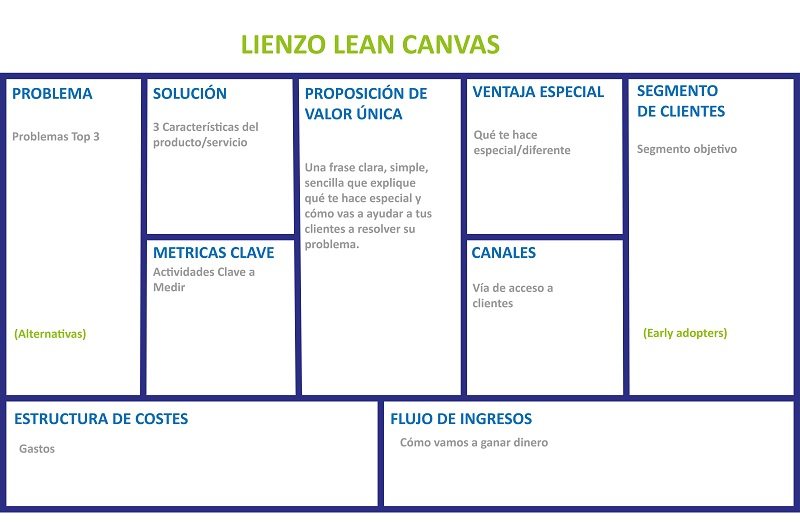
\includegraphics[scale=0.6]{imagenes/leanCanvas.jpg}
\caption{Lean canvas}
\label{leanCanvas}
\end{center}
\end{figure}

Estas hipótesis no conforman el modelo de negocio definivo, si no que irán evolucionando a lo largo de la vida de la empresa de acuerdo al feedback de los clientes. Esta evolución del producto en relación a los deseos del clientes se denomina \textbf{customer development} y es uno de los conceptos claves en Lean startup.

El ciclo de vida de una startup se basa en tres pasos fundamentales que se repiten cíclicamente:
\begin{itemize}
	\item Construir: se diseña el producto en función de las hipótesis que se establecen en el \textbf{lean canvas}. En la primera iteración se crea una versión del producto que tenga las minímas funcionalidades necesarias para aportar valor a los potenciales clientes. Esta versión del producto se denomina \textbf{producto minímo viable}. El objetivo de esta etapa es ''comenzar a recopilar datos y medir resultados. Este modelo de producto no busca ser el resultado final sino un producto suficiente para testar la reacción del potencial cliente" \cite{antevenio2016}.
	\item Medir: tras contrastar nuestras hipótesis de negocio con los clientes a través del \textbf{producto minímo viable} obtenemos información sobre nuestro producto y sobre la propia empresa mediante \textbf{métricas clave}. Dichas métricas (tales como ¿Cuánto cuesta captar un cliente? o ¿Cuánto dinero gastamos mensualmente?) son valoraciones objetivas sobre el rendimiento del producto y de la empresa, y calcularlas de forma periódica es importante ya que permite trazar una evolución y detectar errores y mejoras en la estrategia empresarial.
	\item Aprender: es una etapa clave ya que si el conocimiento obtenido se aplica, se estará más cerca de crear un producto que los clientes quieran comprar. ''este conocimiento adquirido se debe aplicar a un nuevo proceso que comienza de nuevo. Se vuelve a crear un producto, que será una mejora del mismo lo que hace arrancar de nuevo el círculo de crear, medir y aprender" \cite{antevenio2016}. Al llegar a este punto las startups se deben plantear si realizar un pequeño ajuste al producto y volver a \textbf{iterar} o si bien, en caso de que los resultados del producto hayan sido un desastre, hacer cambios de base al modelo de negocio. Estos cambios que afectan a una o más hipótesis del \textbf{lean canvas} se denominan \textbf{pivotar} y consisten en ''cambiar una hipótesis fundamental sobre el producto, la estrategia, y el motor de crecimiento" \cite{emooc}.
\end{itemize}

El proceso se puede realizar cuantas veces sea necesario hasta conseguir el producto que se considere más acorde al cliente. La metodología Lean Startup no trata de evitar que fallemos en el primer intento de lanzar al mercado nuestro servicio, sino que trata de que ese fallo nos salga más ‘barato’ al haber empleado una cantidad considerablemente menor de tiempo y de recursos materiales y económicos \cite{andreapelaez} .






\chapter{Marco Teórico}
\label{marcoteorico}

El contenido de este capítulo es una especie de muestrario de cosas que puedes hacer con \LaTeX.  Por ejemplo, incluir una cita bibliográfica   \cite{BOE_IM_UA} dentro del texto. En esta página de demostración también puedes encontrar información útil acerca de cómo escribir con  \LaTeX.\footnote{En http://metodos.fam.cie.uva.es/~latex/apuntes/apuntes.html hay unos buenos apuntes al respecto.}

Hacer una lista es simple en \LaTeX. Para ello has de crear un entorno (así se llama) itemize con
\begin{verbatim}
\begin{itemize}
...
\end{itemize}
\end{verbatim}
Y dentro de esa estructura, añadir cada elemento de la lista precedido de 
\begin{verbatim}
\item primer item de lista
\item segundo item de lista
...
\item ultimo item de lista
\end{verbatim}
\section{Elaboración de listas.}

Es importante que revises este texto tal como aparece en la plantilla y relaciones el aspecto que tiene el PDF final con cómo está escrito el documento \LaTeX.

Aquí va una lista:
\begin{itemize}
    \item Ingeniería Informática.
    \item Ingeniería Sonido e Imagen en Telecomunicación.
    \item Ingeniería Multimedia.
    \begin{itemize}
         \item Mención: Creación y ocio digital.
         \item Mención: Gestión de Contenidos.
    \end{itemize}
\end{itemize}

Ahora veremos otra estructura más: las tablas.

\section{Inserción de tablas}

Aquí va una tabla\footnote{En http://www.tablesgenerator.com/ se puede encontrar un generador On-Line de tablas para \LaTeX} para que se vea cómo insertar una tabla simple dentro del documento.

\begin{table}[h]
\begin{center}
\begin{tabular}{lllll}
&columna A&columna B&columna C\\
\hline
fila 1&fila 1, columna A & fila 1, columna B & fila 1, columna C\\
fila 2&fila 2, columna A & fila 2, columna B & fila 2, columna C\\
fila 3&fila 3, columna A & fila 3, columna B & fila 3, columna C\\ \hline
\end{tabular}
\end{center}
\caption{Ejemplo de tabla.}
\label{tabladeejemplo}
\end{table}

\LaTeX usa un sistema de parámetros para ``decorar'' las tablas. Puedes consultar estos parámetros en la tabla \ref{tabla_parametros} de la página \pageref{tabla_parametros}. La tabla se ubicará donde, a juicio de \LaTeX, menos moleste por lo que puede no aparecer necesariamente donde se ha insertado en el texto original. 

\begin{table}
\begin{center}
\begin{tabular}{|c|p{0.8\textwidth}|}
\hline
Parámetro & \multicolumn{1}{c|}{Significado} \\ \hline
\texttt{h} & Situa el elemento flotante \emph{preferentemente}
(es decir, si es posible) en la situación exacta donde se incluye este \\
\texttt{t} & Situa el elemento en la parte de arriba de la página \\
\texttt{b} & Situa el elemento en la parte de abajo de la página \\
\texttt{p} & Situa el elemento en una página aparte dedicada sólo a
elementos flotantes; en el caso del formato \texttt{article},
ésta se situa al final del documento, mientras que para al book es
colocada al final de cada capítulo \\ \hline
\end{tabular}
\end{center}
\caption{Parámetros optativos de los entornos flotantes}
\label{tabla_parametros}
\end{table}



\section{Inserción de figuras}

Las figuras son un caso un poco especial ya que \LaTeX busca el mejor lugar para ponerlas, no siendo necesariamente el ligar donde está la referencia. Por ello es importante añadirle un ``caption'' y un ``label'' para poder hacer referencia a ellas en el párrafo correspondiente. Nosotros ponemos la referencia a la figura \ref{logo_im} que está en la página \pageref{logo_im}. justo aquí debajo, pero \LaTeX puede que la ubique en otro lugar.

\begin{figure}
\begin{center}

\includegraphics[scale=0.25]{imagenes/logoim.jpg}
\caption{Logo de Ingeniería  Multimedia.}
\label{logo_im}
\end{center}
\end{figure}

\begin{figure}
\begin{center}

\includegraphics[scale=0.25]{imagenes/logoeps.jpg}
\caption{Logo de la EPS.}
\label{logo_eps}
\end{center}
\end{figure}

\section{Inserción de código}
A veces tendrás que insertar algún pedazo de código fuente para explicar algo relacionado con él. No sustituyas explicaciones con enormes listados de código. Si pones algo de código en tu TFG que sea para demostrar algo o explicar alguna solución.

\LaTeX te ayuda a escribir código de manera que su presentación tenga las marcas y tabulaciones propias de este tipo de texto. Para ello, debes poner el código que escribas DENTRO de un entorno  que se llama ``listings''.  La plantilla ya tiene una serie de instrucciones para incluir el paquete ``listings'' y añadirle algunos modificadores por lo que no tienes que incluirlo tú. Simplemente, mete tu código en el entorno ``lstlisting'' y ya está. Puedes indicar el lenguaje en el que está escrito el código y así \LaTeX lo mostrará mejor. Veamos un ejemplo en la figura \ref{C_code}:

Si pones 
\begin{verbatim}
\begin{lstlisting}[style=C, caption={ejemplo código C},label=C_code]
#include <stdio.h>
int main(int argc, char* argv[]) {
  puts("Hola mundo!");
}
\end{lstlisting}
\end{verbatim}

El resultado será:
\begin{lstlisting}[style=C, caption={ejemplo código C},label=C_code]
#include <stdio.h>
int main(int argc, char* argv[]) {
  puts("Hola mundo!");
}
\end{lstlisting}

Por supuesto, puedes mejorar esta presentación utilizando mas modificadores. Esta información y mucha más puede ser encontrada en \cite{listing_packagge} y en \cite{heinz1listings}.

Otro ejemplo, ahora para mostrar código PHP, sería escribir en tu fichero \LaTeX lo siguiente:
\begin{verbatim}
 \begin{lstlisting}[style=PHP, caption={ejemplo código PHP},label=PHP_code]
 /* 
Ejemplo de código en PHP para escribir tu primer programa en este lenguaje
Copia este código en tu ordenador y ejecútalo
*/
<html>
  <head>
    <title>Prueba de PHP</title>
  </head>
  <body>
    <?php echo '<p>Hola Mundo</p>'; ?> //esto lo escribe TODO el mundo
  </body>
</html>
 \end{lstlisting}
\end{verbatim}
 
 y el resultado es: (ver listado \ref{PHP_code})
 
 \begin{lstlisting}[style=PHP, caption={ejemplo código PHP},label=PHP_code]
/* 
Ejemplo de código en PHP para escribir tu primer programa en este lenguaje. Copia este código en tu ordenador y ejecútalo
*/
 <html>
  <head>
    <title>Prueba de PHP</title>
  </head>
  <body>
    <?php echo '<p>Hola Mundo</p>'; ?> //esto lo escribe TODO el mundo
  </body>
</html>
 \end{lstlisting}
 
 Observa cómo \LaTeX ha puesto los comentarios en gris y ajustado el código para que se muestre más claro.
 
 Si quieres añadir código en otros lenguajes, cambia el comando que dice ``style=nombredellenguaje'' por ``languaje=nombredelnuevolenguaje''.
\chapter{Objetivos}

\section{Objetivo principal}

El objetivo principal de este proyecto la creación un videojuego mediante el cual se puedan aprender conceptos claves acerca del emprendimiento y en concreto sobre la metodología \textquote{Lean startup}.


\section{Objetivos específicos}

\begin{itemize}
	\item Emplear el concepto storytelling para diseñar y escribir una historia que se desarrolle a lo largo de conversaciones entre el jugador y los demás personajes.
	\item Implementar un sistema conversacional en el que el jugador pueda seleccionar las respuestas que desea dar y en función de ello cambie la historia.
	\item Crear una interfaz de usuario que cumpla con unos criterios de calidad y que permita al jugador interactuar con la aplicación.
	\item Crear modelos 3D de personajes y otros elementos tales como edificios. Texturizar dichos modelos.
\end{itemize}


\section{Objetivos secundarios}

\begin{itemize}
	\item Crear un videojuego usando el motor de videojuegos \textquote{Unity3D}\footnote{https://unity3d.com/es}.
	\item Planificar el desarrollo de un proyecto de desarrollo de software y llevarlo a cabo.
	\item Aprender nuevas habilidades sobre el motor de videojuegos \textquote{Unity3D} y el lenguaje de programación C\#.
	\item Crear un GDD (documento de diseño de videojuego) donde se documente con precisión como será el juego.
	\item Aprender nuevas habilidades sobre el software de modelado 3D \textquote{Blender}\footnote{https://www.blender.org/}.

\end{itemize}




\chapter{Metodología}

Para la realización del proyecto, la creación del videojuego, se dispondrán de 6 meses que se dividirán de la siguiente forma: inicialmente un mes y medio para la investigación, especificación del producto y planificación; cuatro meses desarrollando el producto; finalmente medio mes para dar los últimos retoques al juego y lanzar una versión beta.

Para el desarrollo del videojuego se utilizará una metodología ágil, ya que al disponer de poco tiempo para el desarrollo se necesitará tener un producto cuanto antes para poder enfrentarlo al público y obtener el feedback de este. Utilizando una metodología ágil se focaliza el esfuerzo en el desarrollo en lugar de en una excesiva planificación. De esta forma 
\begin{itquote}
	se trabaja realizando entregas parciales pero funcionales del producto. De ese modo, es posible entregar en el menor intervalo de tiempo posible una versión funcional del producto.
	\begin{flushright}
	 	\cite{eduardomartinez2014}.
 	\end{flushright}
\end{itquote}

Además la utilización de estas metodologías ayuda enormemente a reducir el riesgo: al crear un videojuego, en este caso educativo, a pesar de las mejores intenciones de los desarrolladores no se puede saber con certeza si será del agrado de los jugadores.

Es por ello que la mejor estrategia posible es crear un producto minimo viable (MVP) y que posteriormente se desarrolle y corrija según los deseos de aquellos que lo jugarán. 

Existen actualmente una gran cantidad de metodologías ágiles. Entre las más populares se pueden destacar: 

\begin{itemize}
	\item Scrum: es una metodología orientada a equipos. Proporciona herramientas para el seguimiento diario del proyecto, la planificación de trabajo de forma iterativa y la comunicación y cooperación de los integrantes del grupo.
	\item Extreme Programming: orientada a equipos con pocos programadores. 
		\begin{itquote}
			se aplica en equipos con muy pocos programadores quienes llevan muy pocos procesos en paralelo. Consiste entonces en diseñar, implementar y programar lo más rápido posible, hasta en casos se recomienda saltar la documentación y los procedimientos tradicionales.
			\begin{flushright}
	 			\cite{opheliapastrana2015}.
 			\end{flushright}
		\end{itquote}
	\item Kanban: esta metodología propone dividir el trabajo en diferentes etapas bien diferenciadas. El objetivo es evitar los cuellos de botella limitando el trabajo en curso. Para ello, se establece un límite de trabajo en curso, lo que obliga a que cuando una tarea se empieza se debe terminar antes de iniciar una nueva.
\end{itemize}

La metodología ágil a utilizar será Kanban ya que es tremendamente sencilla de implementar: con unas simples tarjetas se pueden especificar las tareas a realizar, y con un tablero se pueden crear columnas que representan los estados de las diferentes tareas.

Dada la facilidad con la que se puede implementar Kanban, y que no es un sistema directamente orientado a equipos como SCRUM, será muy adecuado para el proyecto.


En cuanto al producto a desarrollar, los cuatro meses de desarrollo se dividirán en iteraciones de duración variable. Al finalizar la segunda iteración se espera tener un mínimo producto viable (MVP) y en las dos siguientes se perfeccionará dicho producto.

En cuanto al tiempo de desarrollo se dividirá en cuatro iteraciones: 

\begin{itemize}
	\item Primera iteración: desarrollo de la parte software del MVP usando placeholders en lugar de los modelos 3D y los demás elementos gráficos
	\item Segunda iteración: inclusión de los modelos 3D e imágenes definitivas
	\item Tercera iteración: recolección de feedback y corrección de errores. Optimización del juego
	\item Cuarta iteración: recolección de feedback y corrección de errores. Detalles finales del juego
\end{itemize}

Para ilustrar esta distribución de tareas se ha creado un diagrama de Gantt simplificado como se puede apreciar en la siguiente imagen \ref{gantt01}.

\begin{figure}
	\begin{center}
		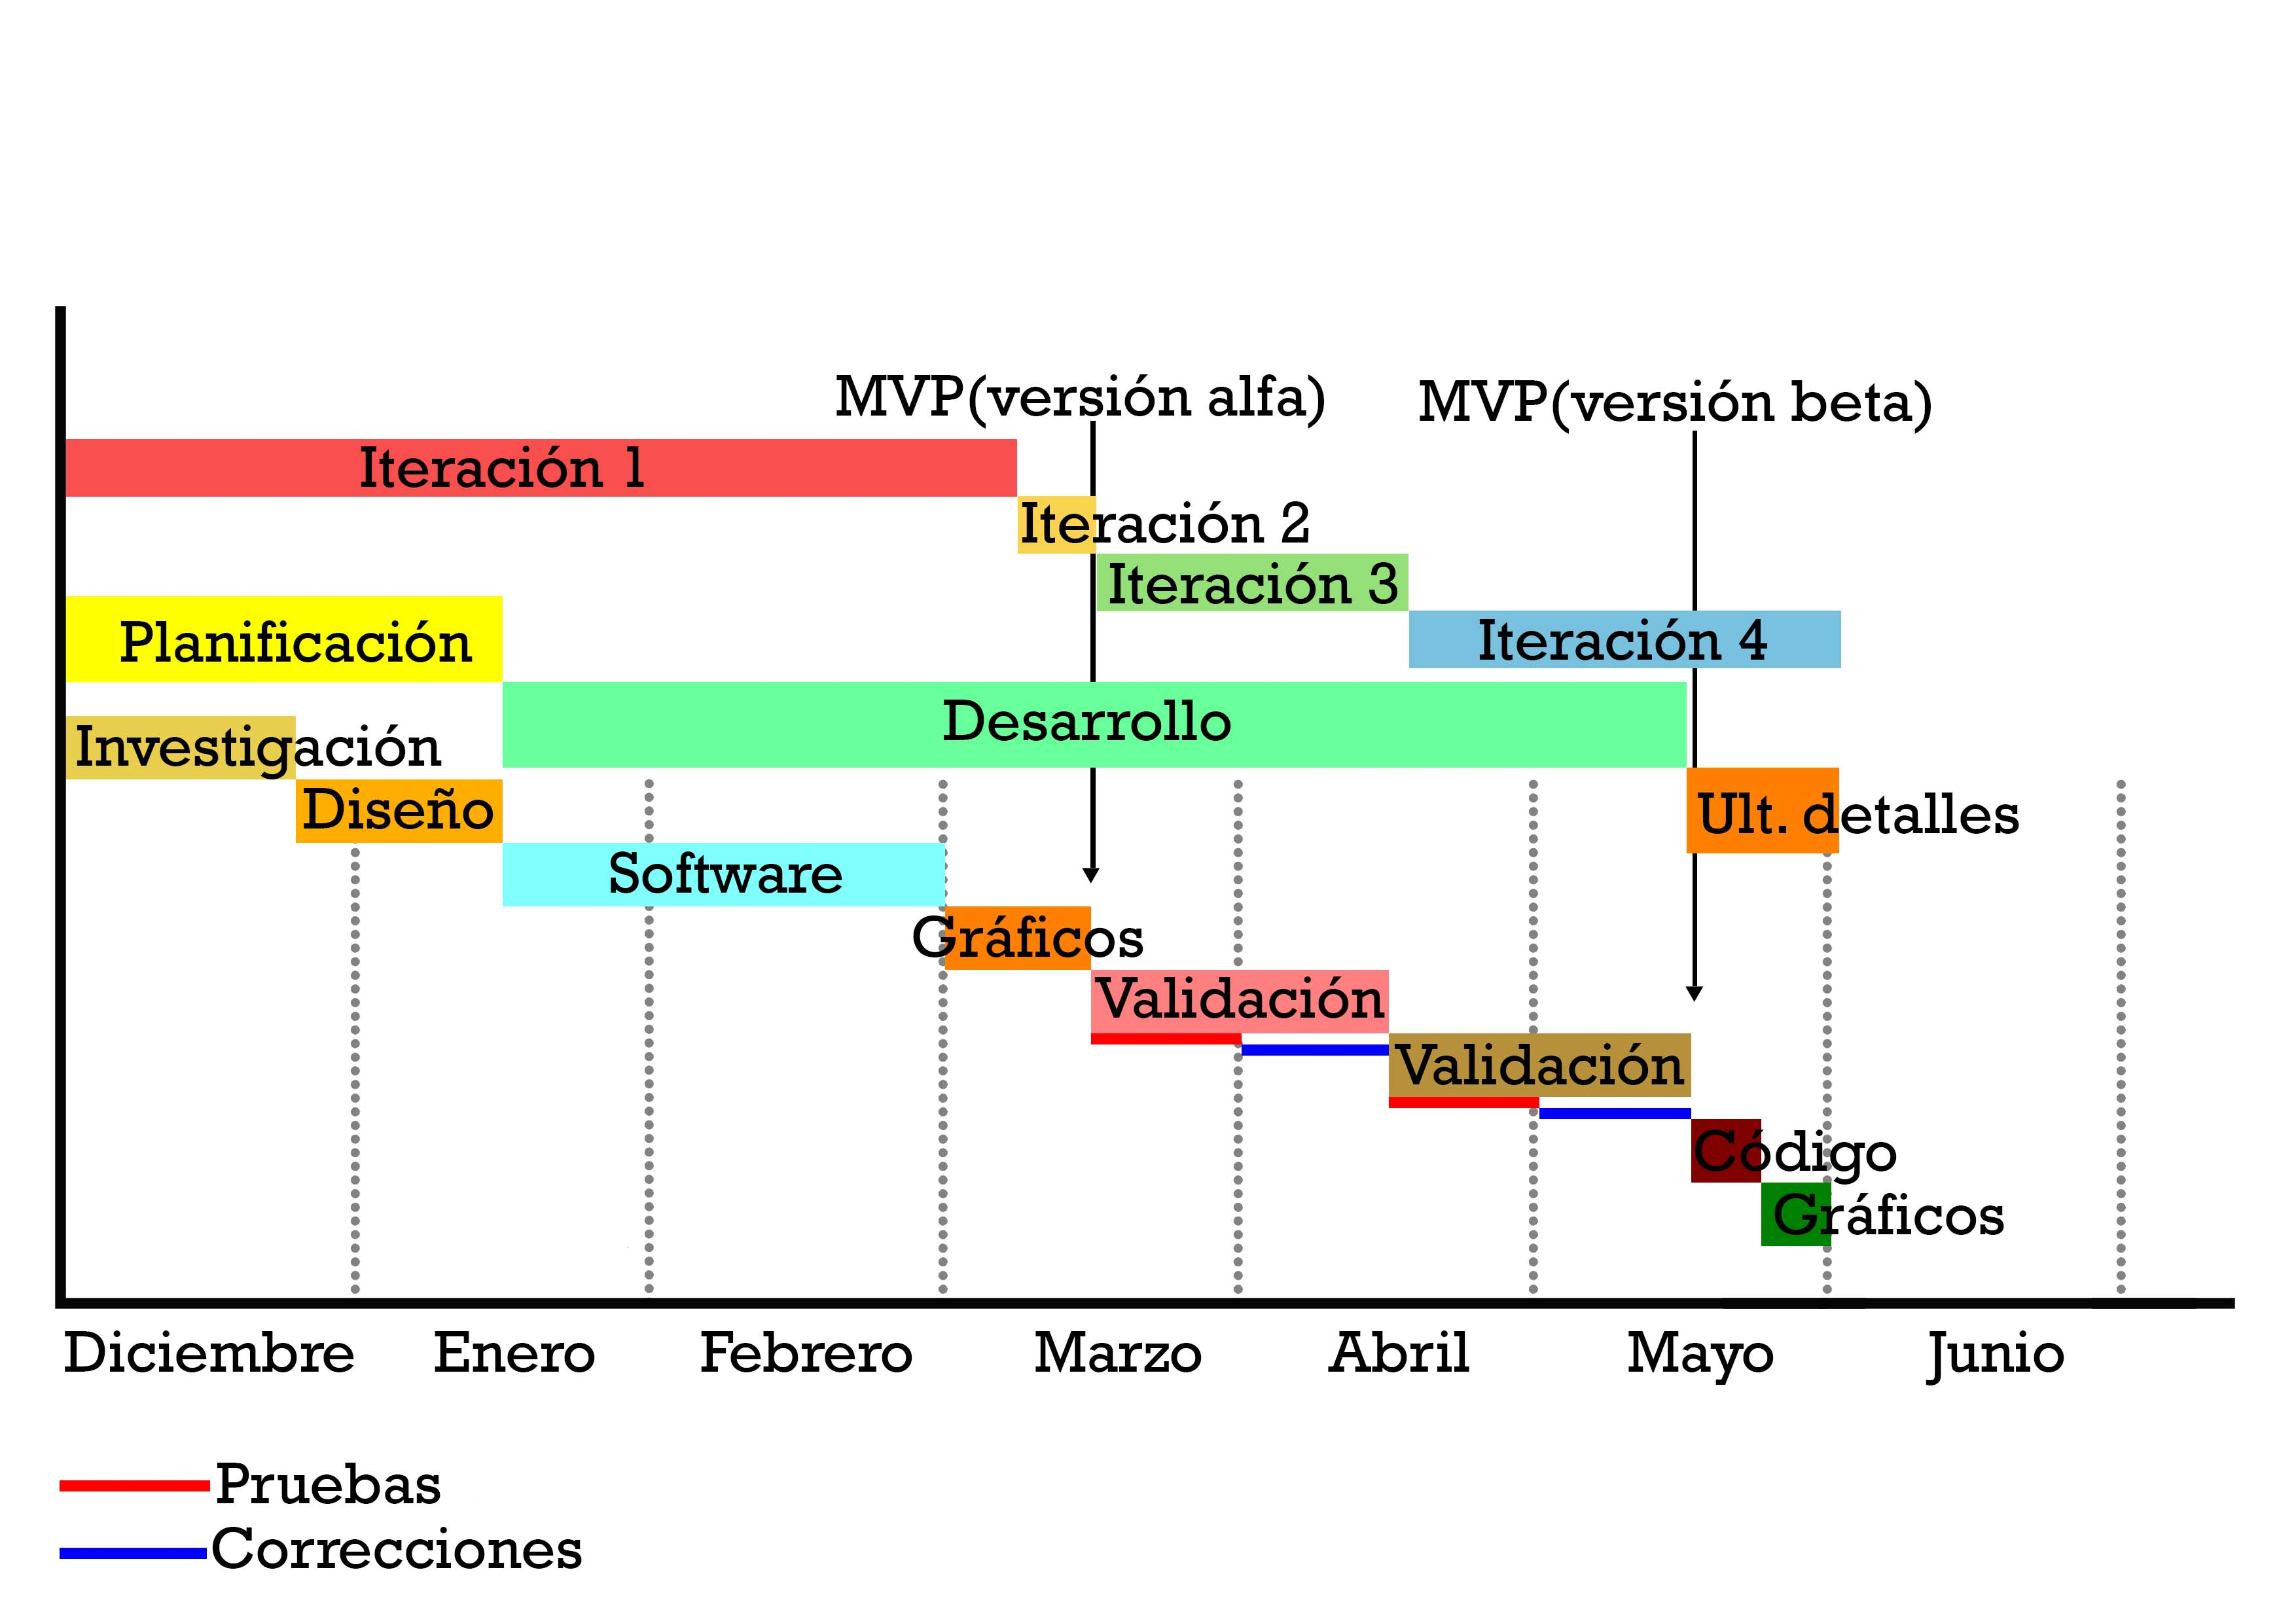
\includegraphics[scale=0.6]{imagenes/GanttDiagram.jpg}
		\caption{Diagrama de Gantt con la distribución temporal y las dependencias de las tareas}
		\label{gantt01}
	\end{center}
\end{figure}

Se utilizará la herramienta online TargetProcess \footnote{www.targetprocess.com} para disponer de un tablero virtual \textquote{Kanban} en el cual poner las tarjetas y separarlas por procesos. En este aspecto goza de más popularidad la herramienta Trello \footnote{https://trello.com/}, aunque TargetProcess es más completa y ofrece muchas opciones como filtros, métricas y otras utilidades para monitorizar el trabajo.

\section{Producción de contenido}
\subsection{Modelos 3D}
Los modelos 3D a utilizar se obtendrán de sitios web que ofrezcan este tipo de recursos de forma gratuita y con licencia que permita su uso comercial. En caso de que alguno de los modelos no se encontrara se modelaría el mismo utilizando el software Blender. 
\subsection{Música y sonidos}

\subsecion{Motor de videojuego}



\chapter{Desarrollo}

\section{Descripción general}

Para describir el desarrollo se ha decidido seguir el estándar IEEE 830 para la especificación de requisitos \footnote{\url{www.fdi.ucm.es/profesor/Gmendez/docs/is0809/ieee830.pdf}}.

\section{Perspectiva del producto}

El sistema a construir consistirá en una aplicación móvil para dispositivos Android \footnote{\url{www.android.com}} desarrollada con el motor de videojuegos Unity3D \footnote{\url{https://unity3d.com/es/}}. 

La aplicación no formará parte de un sistema mayor, será un videojuego totalmente independiente. Aun así se hará uso de servicios de terceros tales como librerías de software, frameworks y APIs entre otros.

\section{Funcionalidad del producto}

Resumen de las funcionalidades principales que el producto debe realizar, sin entrar en información de detalle.
El videojuego deberá permitir el movimiento del jugador en el plano 2D, además podrá interactuar con los NPCs y dialogar con ellos. Se podrán completar objetivos y logros para de este modo avanzar en la historia.

El juego además enseñará conceptos clave sobre \textquote{Lean Startup} y sobre el emprendimiento en general.

\section{Características de los usuarios}

El perfil de un consumidor de formación sobre emprendimiento es muy amplio: desde jóvenes recién graduados llenos de optimismo hasta personas de mediana edad que desean reinventarse y dejar de ser asalariados. 

Es por ello que es difícil concretar un perfil ya que son diferentes personas de diferentes edades y perfiles socioculturales las que desean aventurarse en el emprendimiento.

En cualquier caso sí se pueden encontrar aspectos comunes en esta gran variaded de usuarios:

\begin{itemize}

\item conocimiento tecnológico y como desenvolverse con aplicaciones móviles
\item interés por el mundo del emprendimiento y la empresa
\item interés por los videojuegos
\item interés por los videojuegos educativos

\end{itemize}

\section{Restricciones}

Existen varias limitaciones a tener en cuenta a la hora de diseñar y desarrollar el sistema:

\begin{itemize}

\item para la realización del proyecto se dispondrá de un presupuesto nulo. Es por ello que las herramientas, frameworks y demás productos que se utilicen deberán ser gratuitas.
\item el motor de videojuegos a utilizar deberá ser Unity 3D ya que se tiene conocimiento del mismo y no se dispone de tiempo para aprender a utilizar otro motor de videojuegos.
\item el lenguaje de programación a utilizar será C\# ya que de entre los disponibles para Unity 3D es el más adecuado por potencia, documentación y dominio por parte del desarrollador.
\item el sistema operativo objetivo será Android ya junto con los sistemas operativos para ordenador no requiere ninguna licencia para publicar aplicaciones. La plataforma serán los dispositivos móviles ya que es muy sencillo llegar al público de esta plataforma, aunque no tanto hacerse hueco entre dicha audiencia.

\end{itemize}

\section{Requisitos específicos}

\subsection{Interfaces de usuario}

Respecto a las interfaces de usuario se pueden observar dos estilos claramente diferenciados: las interfaces del menú principal y las de la pantalla de juego. En cuanto a las primeras deberán seguir un estilo minimalista y utilizar controles simples; respecto de las segundas, la simplicidad es obligatoria.

Es un requisito imprescindible que la interfaz mostrada durante el juego no sea intrusiva y entorpezca la experiencia de usuario. Esto se conseguirá disponiendo pequeños botones en la pantalla situados de forma estratégica para que la visión del jugador se centre principalmente en el mundo del juego y los personajes.

Un requisito común de las interfaces de usuario es que debido a que serán mostradas en un dispositivo móvil tendrán que adecuarse a una pantalla pequeña y recibir la interacción del usuario mediante toques en la pantalla del dispositivo.

\subsection{Requisitos funcionales}

Para describir las funcionalidades del sistema se utilizará una aproximación basada en mecánicas. Cada posible acción del usuario sobre el sistema se considerará una mecánica y se definirá como un requisito. 

Dichas mecánicas son activadas al detectarse cierto estímulo. Por ejemplo al producir el estímulo de tocar en algun lugar del mundo, se desencadena la mecánica de movimiento.

Al identificador de cada funcionalidad le acompañarán unas siglas (USR, UI, SYS) dependiendo de si dicha funcionalidad se refiere a mecánicas del usuario, la interfaz de usuario o al sistema.

\subsection{Requisitos de usuario}
\label{requisitosUsuario}

\begin{table}[H]
\centering
\label{my-label}
\begin{tabular}{|l|l|}
\hline
\textbf{Identificador} & RF-USR-01                                                                                                                                                              \\ \hline
\textbf{Nombre}        & Mover personaje                                                                                                                                                        \\ \hline
\textbf{Requerimiento} & El usuario podrá elegir donde mover al personaje controlado                                                                                                            \\ \hline
\textbf{Descripción}   & \begin{tabular}[c]{@{}l@{}}Al tocar con el dedo en cualquier punto de la pantalla el personaje\\   controlado se moverá a esa posición (solo en el eje x)\end{tabular} \\ \hline
\textbf{Prioridad}     & Imprescindible                                                                                                                                                         \\ \hline
\end{tabular}
\end{table}

\begin{table}[H]
\centering
\label{my-label}
\begin{tabular}{|l|l|}
\hline
\textbf{Identificador} & RF-USR-02                                                                                                                                           \\ \hline
\textbf{Nombre}        & Interactuar con NPCs                                                                                                                                \\ \hline
\textbf{Requerimiento} & El usuario podrá seleccionar un NPC con el que interactuar                                                                                          \\ \hline
\textbf{Descripción}   & \begin{tabular}[c]{@{}l@{}}Al tocar con el dedo sobre un NPC, si se está lo suficientemente cerca se\\   abrirá el menú conversacional\end{tabular} \\ \hline
\textbf{Prioridad}     & Imprescindible                                                                                                                                      \\ \hline
\end{tabular}
\end{table}

\begin{table}[H]
\centering
\label{my-label}
\begin{tabular}{|l|l|}
\hline
\textbf{Identificador} & RF-USR-03                                                                                                                                      \\ \hline
\textbf{Nombre}        & Cambiar de escenario                                                                                                                           \\ \hline
\textbf{Requerimiento} & Se podrá navegar entre escenarios                                                                                                              \\ \hline
\textbf{Descripción}   & \begin{tabular}[c]{@{}l@{}}Al clicar en una de las puertas de cada escenario se avanzará al\\   escenario asociado a dicha puerta\end{tabular} \\ \hline
\textbf{Prioridad}     & Imprescindible                                                                                                                                 \\ \hline
\end{tabular}
\end{table}

\subsection{Requisitos de interfaz}

\begin{table}[H]
\centering
\label{my-label}
\begin{tabular}{|l|l|}
\hline
\textbf{Identificador} & RF-UI-01                                                                                                                                                \\ \hline
\textbf{Nombre}        & Navegar menú principal                                                                                                                                  \\ \hline
\textbf{Requerimiento} & Se podrá cambiar entre las diferentes pantallas del menú principal                                                                                      \\ \hline
\textbf{Descripción}   & \begin{tabular}[c]{@{}l@{}}Arrastrando con el dedo en la pantalla hacia la derecha/izquierda se\\   cambiará a la correspondiente pantalla\end{tabular} \\ \hline
\textbf{Prioridad}     & Imprescindible                                                                                                                                          \\ \hline
\end{tabular}
\end{table}

\begin{table}[H]
\centering
\label{my-label}
\begin{tabular}{|l|l|}
\hline
\textbf{Identificador} & RF-UI-02                                                                                                                                        \\ \hline
\textbf{Nombre}        & Comenzar juego                                                                                                                                  \\ \hline
\textbf{Requerimiento} & \begin{tabular}[c]{@{}l@{}}Se empezará el juego al seleccionar el botón correspondiente en el menú\\   principal\end{tabular}                   \\ \hline
\textbf{Descripción}   & \begin{tabular}[c]{@{}l@{}}En el el menú principal en la vista inicial se podrá comenzar el juego al\\   presionar el botón "play"\end{tabular} \\ \hline
\textbf{Prioridad}     & Imprescindible                                                                                                                                  \\ \hline
\end{tabular}
\end{table}

\begin{table}[H]
\centering
\label{my-label}
\begin{tabular}{|l|l|}
\hline
\textbf{Identificador} & RF-UI-03                                                                                                                            \\ \hline
\textbf{Nombre}        & Desactivar/Activar música                                                                                                           \\ \hline
\textbf{Requerimiento} & Se podrá desactivar la música ambiente del juego                                                                                    \\ \hline
\textbf{Descripción}   & \begin{tabular}[c]{@{}l@{}}Clicando en el icono de Música en el menú de opciones se\\   activará/desactivará la música\end{tabular} \\ \hline
\textbf{Prioridad}     & Baja                                                                                                                                \\ \hline
\end{tabular}
\end{table}

\begin{table}[H]
\centering
\label{my-label}
\begin{tabular}{|l|l|}
\hline
\textbf{Identificador} & RF-UI-04                                                                                                                                           \\ \hline
\textbf{Nombre}        & Desactivar/Activar sonidos                                                                                                                         \\ \hline
\textbf{Requerimiento} & Se podrán desactivar los efectos de sonido del juego                                                                                               \\ \hline
\textbf{Descripción}   & \begin{tabular}[c]{@{}l@{}}Clicando en el icono de Sonidos en el menú de opciones se\\   activarán/desactivarán los efectos de sonido\end{tabular} \\ \hline
\textbf{Prioridad}     & Baja                                                                                                                                               \\ \hline
\end{tabular}
\end{table}

\begin{table}[H]
\centering
\label{my-label}
\begin{tabular}{|l|l|}
\hline
\textbf{Identificador} & RF-UI-05                                                                                                                                          \\ \hline
\textbf{Nombre}        & Eliminar logros                                                                                                                                   \\ \hline
\textbf{Requerimiento} & Se podrán eliminar los logros conseguidos                                                                                                         \\ \hline
\textbf{Descripción}   & \begin{tabular}[c]{@{}l@{}}Clicando en el icono de Eliminar logros del menú de opciones se\\   eliminarán todos los logros obtenidos\end{tabular} \\ \hline
\textbf{Prioridad}     & Baja                                                                                                                                              \\ \hline
\end{tabular}
\end{table}

\begin{table}[H]
\centering
\label{my-label}
\begin{tabular}{|l|l|}
\hline
\textbf{Identificador} & RF-UI-06                                                                                                                                                              \\ \hline
\textbf{Nombre}        & Ver otros juegos                                                                                                                                                      \\ \hline
\textbf{Requerimiento} & Se podrá acceder a la descarga de otros juegos del autor                                                                                                              \\ \hline
\textbf{Descripción}   & \begin{tabular}[c]{@{}l@{}}Clicando en los iconos de juegos del apartado "Mas juegos" se\\   accederá a Google Play donde se podrá descargar dicho juego\end{tabular} \\ \hline
\textbf{Prioridad}     & Baja                                                                                                                                                                  \\ \hline
\end{tabular}
\end{table}

\begin{table}[H]
\centering
\label{my-label}
\begin{tabular}{|l|l|}
\hline
\textbf{Identificador} & RF-UI-07                                                                                                                                                                           \\ \hline
\textbf{Nombre}        & Navegar entre logros                                                                                                                                                               \\ \hline
\textbf{Requerimiento} & Se podrán seleccionar logros y ver su descripción                                                                                                                                  \\ \hline
\textbf{Descripción}   & \begin{tabular}[c]{@{}l@{}}En el menú de logros se podrá navegar entre los logros usando las flechas\\   de navegación y ver la descripción y la imagen de los mismos\end{tabular} \\ \hline
\textbf{Prioridad}     & Media                                                                                                                                                                              \\ \hline
\end{tabular}
\end{table}

\begin{table}[H]
\centering
\label{my-label}
\begin{tabular}{|l|l|}
\hline
\textbf{Identificador} & RF-UI-08                                                                                                                                                                    \\ \hline
\textbf{Nombre}        & Ver logros desbloquados                                                                                                                                                     \\ \hline
\textbf{Requerimiento} & Se podrá ver la cantidad de logros desbloqueados hasta el momento                                                                                                           \\ \hline
\textbf{Descripción}   & \begin{tabular}[c]{@{}l@{}}En el menú de logros aparecerá un texto representando el número de logros\\   desbloqueados hasta el momento y el total a conseguir\end{tabular} \\ \hline
\textbf{Prioridad}     & Baja                                                                                                                                                                        \\ \hline
\end{tabular}
\end{table}

\begin{table}[H]
\centering
\label{my-label}
\begin{tabular}{|l|l|}
\hline
\textbf{Identificador} & RF-UI-09                                                                                                                  \\ \hline
\textbf{Nombre}        & Ver descripción de logro                                                                                                  \\ \hline
\textbf{Requerimiento} & Se podrá ver una descripción de los logros                                                                                \\ \hline
\textbf{Descripción}   & \begin{tabular}[c]{@{}l@{}}En el menú de logros se podrá ver un texto descriptivo del logro\\   seleccionado\end{tabular} \\ \hline
\textbf{Prioridad}     & Media                                                                                                                     \\ \hline
\end{tabular}
\end{table}

\begin{table}[H]
\centering
\label{my-label}
\begin{tabular}{|l|l|}
\hline
\textbf{Identificador} & RF-UI-10                                                                                                                                                                                                               \\ \hline
\textbf{Nombre}        & Navegar entre logros                                                                                                                                                                                                   \\ \hline
\textbf{Requerimiento} & Se podrá seleccionar el logro del que se desea ver información                                                                                                                                                         \\ \hline
\textbf{Descripción}   & \begin{tabular}[c]{@{}l@{}}En el menú de logros se podrá navegar entre logros tocando y arrastrando\\   en la lista de logros. El logro que se sitúe en el centro de la pantalla será\\   el logro activo\end{tabular} \\ \hline
\textbf{Prioridad}     & Media                                                                                                                                                                                                                  \\ \hline
\end{tabular}
\end{table}

\begin{table}[H]
\centering
\label{my-label}
\begin{tabular}{|l|l|}
\hline
\textbf{Identificador} & RF-UI-11                                                                                                                                                                                                                                         \\ \hline
\textbf{Nombre}        & Abrir selector de personaje                                                                                                                                                                                                                      \\ \hline
\textbf{Requerimiento} & Se podrá abrir un menú donde seleccionar el personaje a controlar                                                                                                                                                                                \\ \hline
\textbf{Descripción}   & \begin{tabular}[c]{@{}l@{}}Clicando en el icono del selector de personaje se abrirá una ventana con\\   los iconos de cada personaje. El icono del personaje actualmente controlado\\   se mostrará en gris y no será seleccionable\end{tabular} \\ \hline
\textbf{Prioridad}     & Imprescindible                                                                                                                                                                                                                                   \\ \hline
\end{tabular}
\end{table}

\begin{table}[H]
\centering
\label{my-label}
\begin{tabular}{|l|l|}
\hline
\textbf{Identificador} & RF-UI-12                                                                                                                                                                                                                 \\ \hline
\textbf{Nombre}        & Seleccionar personaje                                                                                                                                                                                                    \\ \hline
\textbf{Requerimiento} & Al clicar en un icono de personaje se cambiará el personaje seleccionado                                                                                                                                                 \\ \hline
\textbf{Descripción}   & \begin{tabular}[c]{@{}l@{}}Al clicar en uno de los iconos de personaje se cambia el personaje\\   controlado. En el icono del selector de personaje aparecerá el icono del\\   nuevo personaje seleccionado\end{tabular} \\ \hline
\textbf{Prioridad}     & Imprescindible                                                                                                                                                                                                           \\ \hline
\end{tabular}
\end{table}

\begin{table}[H]
\centering
\label{my-label}
\begin{tabular}{|l|l|}
\hline
\textbf{Identificador} & RF-UI-13                                                              \\ \hline
\textbf{Nombre}        & Cerrar selector de personaje                                          \\ \hline
\textbf{Requerimiento} & Se podrá cerrar el menú donde seleccionar el personaje a controlar    \\ \hline
\textbf{Descripción}   & Clicando en el selector de personaje, si este está abierto se cerrará \\ \hline
\textbf{Prioridad}     & Imprescindible                                                        \\ \hline
\end{tabular}
\end{table}

\begin{table}[H]
\centering
\label{my-label}
\begin{tabular}{|l|l|}
\hline
\textbf{Identificador} & RF-UI-14                                                                                                                                                                                                                        \\ \hline
\textbf{Nombre}        & Notificar objetivo completado                                                                                                                                                                                                   \\ \hline
\textbf{Requerimiento} & Cuando se cumpla el objetivo actual se mostrará una notificación                                                                                                                                                                \\ \hline
\textbf{Descripción}   & \begin{tabular}[c]{@{}l@{}}Al completar un objetivo el icono del indicador de objetivos girará. El\\   texto del nuevo objetivo se añadirá a la lista de objetivos. El objetivo\\   completado se mostrará tachado\end{tabular} \\ \hline
\textbf{Prioridad}     & Media                                                                                                                                                                                                                           \\ \hline
\end{tabular}
\end{table}

\begin{table}[H]
\centering
\label{my-label}
\begin{tabular}{|l|l|}
\hline
\textbf{Identificador} & RF-UI-15                                                                                                                                                                                    \\ \hline
\textbf{Nombre}        & Abrir indicador de objetivos                                                                                                                                                                \\ \hline
\textbf{Requerimiento} & Se podrá abrir la lista de objetivos                                                                                                                                                        \\ \hline
\textbf{Descripción}   & \begin{tabular}[c]{@{}l@{}}Al clicar en el icono del indicador de objetivos se desplegará una lista\\   con los objetivos completados tachados y el objetivo actual sin tachar\end{tabular} \\ \hline
\textbf{Prioridad}     & Media                                                                                                                                                                                       \\ \hline
\end{tabular}
\end{table}

\begin{table}[H]
\centering
\label{my-label}
\begin{tabular}{|l|l|}
\hline
\textbf{Identificador} & RF-UI-16                                                                                                                                \\ \hline
\textbf{Nombre}        & Cerrar indicador de objetivos                                                                                                           \\ \hline
\textbf{Requerimiento} & Se podrá cerrar la lista de objetivos                                                                                                   \\ \hline
\textbf{Descripción}   & \begin{tabular}[c]{@{}l@{}}Al clicar en el icono del indicador de objetivos se cerrará la lista si\\   esta estaba abierta\end{tabular} \\ \hline
\textbf{Prioridad}     & Media                                                                                                                                   \\ \hline
\end{tabular}
\end{table}

\begin{table}[H]
\centering
\label{my-label}
\begin{tabular}{|l|l|}
\hline
\textbf{Identificador} & RF-UI-17                                                                                                                                                                                                                                       \\ \hline
\textbf{Nombre}        & Abrir menú conversacional                                                                                                                                                                                                                      \\ \hline
\textbf{Requerimiento} & Se abrirá el menú conversacional al interactuar con un personaje                                                                                                                                                                               \\ \hline
\textbf{Descripción}   & \begin{tabular}[c]{@{}l@{}}Al abrir el menú conversacional se hará zoom sobre los personajes\\   involucrados. Se mostrará un texto en la pantalla correspondiente a lo que\\   dice el NPC y botones con las posibles respuestas\end{tabular} \\ \hline
\textbf{Prioridad}     & Imprescindible                                                                                                                                                                                                                                 \\ \hline
\end{tabular}
\end{table}

\begin{table}[H]
\centering
\label{my-label}
\begin{tabular}{|l|l|}
\hline
\textbf{Identificador} & RF-UI-18                                                                                                                         \\ \hline
\textbf{Nombre}        & Contestar NPC                                                                                                                    \\ \hline
\textbf{Requerimiento} & Se podrá contestar a los NPC usando el menú conversacional                                                                       \\ \hline
\textbf{Descripción}   & \begin{tabular}[c]{@{}l@{}}Clicando en uno de los botones se contestará al NPC y se actualizará la\\   conversación\end{tabular} \\ \hline
\textbf{Prioridad}     & Imprescindible                                                                                                                   \\ \hline
\end{tabular}
\end{table}

\begin{table}[H]
\centering
\label{my-label}
\begin{tabular}{|l|l|}
\hline
\textbf{Identificador} & RF-UI-19                                                                                                                                                                                                                                                                                             \\ \hline
\textbf{Nombre}        & Terminar conversación                                                                                                                                                                                                                                                                                \\ \hline
\textbf{Requerimiento} & \begin{tabular}[c]{@{}l@{}}Al alcanzar cierto punto de la conversación se cerrará el menu\\   conversacional\end{tabular}                                                                                                                                                                            \\ \hline
\textbf{Descripción}   & \begin{tabular}[c]{@{}l@{}}Cuando la última decisión tomada tiene asociada tiene la marca\\   correspondiente de fin de conversación el menú conversacional se cerrará. El\\   punto en el que se encuentra la conversación se guarda para retomarla desde\\   ese punto posteriormente\end{tabular} \\ \hline
\textbf{Prioridad}     & Imprescindible                                                                                                                                                                                                                                                                                       \\ \hline
\end{tabular}
\end{table}

\subsection{Requisitos de sistema}

\begin{table}[H]
\centering
\label{my-label}
\begin{tabular}{|l|l|}
\hline
\textbf{Identificador} & RF-SYS-01                                                                                                                                                    \\ \hline
\textbf{Nombre}        & Iniciar menú principal                                                                                                                                       \\ \hline
\textbf{Requerimiento} & \begin{tabular}[c]{@{}l@{}}Al iniciar el juego el menú principal comienza en la vista\\   correspondiente\end{tabular}                                       \\ \hline
\textbf{Descripción}   & \begin{tabular}[c]{@{}l@{}}Al iniciar el juego el menú principal mostrará la vista con el título\\   principal y el botón para iniciar el juego\end{tabular} \\ \hline
\textbf{Prioridad}     & Imprescindible                                                                                                                                               \\ \hline
\end{tabular}
\end{table}

\begin{table}[H]
\centering
\label{my-label}
\begin{tabular}{|l|l|}
\hline
\textbf{Identificador} & RF-SYS-02                                                                                                                                                                                                                                         \\ \hline
\textbf{Nombre}        & Seleccionar personaje                                                                                                                                                                                                                             \\ \hline
\textbf{Requerimiento} & \begin{tabular}[c]{@{}l@{}}Al clicar en un icono del selector de personaje se cambiará el personaje\\   controlado\end{tabular}                                                                                                                   \\ \hline
\textbf{Descripción}   & \begin{tabular}[c]{@{}l@{}}Cuando se clique en un icono del selector de personaje se moverá la\\   cámara hasta enfocar al nuevo personaje seleccionado. Cuando se clique en la\\   pantalla se moverá el nuevo personaje controlado\end{tabular} \\ \hline
\textbf{Prioridad}     & Imprescindible                                                                                                                                                                                                                                    \\ \hline
\end{tabular}
\end{table}

\begin{table}[H]
\centering
\label{my-label}
\begin{tabular}{|l|l|}
\hline
\textbf{Identificador} & RF-SYS-03                                                                                                                                                                                                                                                   \\ \hline
\textbf{Nombre}        & Cargar conversación                                                                                                                                                                                                                                         \\ \hline
\textbf{Requerimiento} & Se cargarán las conversaciones desde archivos de texto                                                                                                                                                                                                      \\ \hline
\textbf{Descripción}   & \begin{tabular}[c]{@{}l@{}}Al abrir el menú conversacional se cargará el fichero de texto\\   correspondiente a la conversación del personaje. Si ya se ha conversado con\\   ese personaje se cargará la conversación desde el punto guardado\end{tabular} \\ \hline
\textbf{Prioridad}     & Imprescindible                                                                                                                                                                                                                                              \\ \hline
\end{tabular}
\end{table}

\begin{table}[H]
\centering
\label{my-label}
\begin{tabular}{|l|l|}
\hline
\textbf{Identificador} & RF-SYS-04                                                                                                                                                                        \\ \hline
\textbf{Nombre}        & Contestar NPC                                                                                                                                                                    \\ \hline
\textbf{Requerimiento} & Al contestar a un NPC se actualizarán las respuestas y el texto del NPC                                                                                                          \\ \hline
\textbf{Descripción}   & \begin{tabular}[c]{@{}l@{}}Al contestar a un NPC se leerá del JSON el nuevo texto y las nuevas\\   respuestas y se actualizará la interfaz para mostrar estos datos\end{tabular} \\ \hline
\textbf{Prioridad}     & Imprescindible                                                                                                                                                                   \\ \hline
\end{tabular}
\end{table}

\begin{table}[H]
\centering
\label{my-label}
\begin{tabular}{|l|l|}
\hline
\textbf{Identificador} & RF-SYS-05                                                                                                                                                                                                                                                                                                                 \\ \hline
\textbf{Nombre}        & Codificar conversaciones                                                                                                                                                                                                                                                                                                  \\ \hline
\textbf{Requerimiento} & \begin{tabular}[c]{@{}l@{}}Las conversaciones estarán codificadas en formato JSON y guardadas en\\   ficheros de texto\end{tabular}                                                                                                                                                                                       \\ \hline
\textbf{Descripción}   & \begin{tabular}[c]{@{}l@{}}Cada NPC tendrá un fichero de texto asociado con la conversación que\\   ofrece en formato JSON. Los elementos del JSON serán nodos con texto y nodos\\   hijos con las respuestas asociadas a ese texto. Las respuestas podrán tener\\   "markups" asociadas que indican eventos\end{tabular} \\ \hline
\textbf{Prioridad}     & Imprescindible                                                                                                                                                                                                                                                                                                            \\ \hline
\end{tabular}
\end{table}

\begin{table}[H]
\centering
\label{my-label}
\begin{tabular}{|l|l|}
\hline
\textbf{Identificador} & RF-SYS-06                                                                                                                                                 \\ \hline
\textbf{Nombre}        & Completar objetivo                                                                                                                                        \\ \hline
\textbf{Requerimiento} & \begin{tabular}[c]{@{}l@{}}Se completarán objetivos al tomar decisiones con la markup\\   correspondiente\end{tabular}                                    \\ \hline
\textbf{Descripción}   & \begin{tabular}[c]{@{}l@{}}Cuando se elige una opción de conversación con la "markup" de\\   objetivo asociada, se completará dicho objetivo\end{tabular} \\ \hline
\textbf{Prioridad}     & Imprescindible                                                                                                                                            \\ \hline
\end{tabular}
\end{table}

\begin{table}[H]
\centering
\label{my-label}
\begin{tabular}{|l|l|}
\hline
\textbf{Identificador} & RF-SYS-07                                                                                                                                                                                                               \\ \hline
\textbf{Nombre}        & Cambiar de escenario                                                                                                                                                                                                    \\ \hline
\textbf{Requerimiento} & Cuando el jugador cambia de escenario se modifica la escena                                                                                                                                                             \\ \hline
\textbf{Descripción}   & \begin{tabular}[c]{@{}l@{}}Cuando se produzca un cambio de escenario se desactivará de la escena el\\   escenario abandonado y el jugador aparecerá en el punto de "spawn"\\   asociado al nuevo escenario\end{tabular} \\ \hline
\textbf{Prioridad}     & Imprescindible                                                                                                                                                                                                          \\ \hline
\end{tabular}
\end{table}

\begin{table}[H]
\centering
\label{my-label}
\begin{tabular}{|l|l|}
\hline
\textbf{Identificador} & RF-SYS-08                                                                                                                                                               \\ \hline
\textbf{Nombre}        & Guardar juego                                                                                                                                                           \\ \hline
\textbf{Requerimiento} & El estado del juego se guardará al salir                                                                                                                                \\ \hline
\textbf{Descripción}   & \begin{tabular}[c]{@{}l@{}}Cuando el usuario salga de la aplicación o al menú principal, el estado\\   del juego se guardará en la memoria del dispositivo\end{tabular} \\ \hline
\textbf{Prioridad}     & Baja                                                                                                                                                                    \\ \hline
\end{tabular}
\end{table}

\begin{table}[H]
\centering
\label{my-label}
\begin{tabular}{|l|l|}
\hline
\textbf{Identificador} & RF-SYS-09                                                                                                                                                                                                                    \\ \hline
\textbf{Nombre}        & Cargar juego                                                                                                                                                                                                                 \\ \hline
\textbf{Requerimiento} & Al iniciar el juego se cargarán las partidas guardadas                                                                                                                                                                       \\ \hline
\textbf{Descripción}   & \begin{tabular}[c]{@{}l@{}}Cuando se inice el juego se cargarán las partidas guardadas en caso de\\   existan. De ser así, al iniciar la partida el mundo se encontrará en el\\   estado de la partida guardada\end{tabular} \\ \hline
\textbf{Prioridad}     & Baja                                                                                                                                                                                                                         \\ \hline
\end{tabular}
\end{table}

\begin{table}[H]
\centering
\label{my-label}
\begin{tabular}{|l|l|}
\hline
\textbf{Identificador} & RF-SYS-10                                                                                                                                                                                                                                                                            \\ \hline
\textbf{Nombre}        & Actualizar conversaciones                                                                                                                                                                                                                                                            \\ \hline
\textbf{Requerimiento} & Al completar un objetivo se actualizan las conversaciones                                                                                                                                                                                                                            \\ \hline
\textbf{Descripción}   & \begin{tabular}[c]{@{}l@{}}Al completar un objetivo en una conversación, todas las demás\\   conversaciones se actualizarán a un punto correspondiente de la misma para\\   reflejar el objetivo completado. Las nuevas conversaciones empezarán desde\\   dicho punto.\end{tabular} \\ \hline
\textbf{Prioridad}     & Imprescindible                                                                                                                                                                                                                                                                       \\ \hline
\end{tabular}
\end{table}

\section{Requisitos no funcionales}

\begin{itemize}

\item Rendimiento: el sistema debe de proporcionar una experiencia de juego óptima. Para ello el flujo de juego debe de ser fluido, sin parones o interrupciones.
\item Usabilidad: el sistema debe de ser sencillo de utilizar. De modo que personas sin un contacto o entrenamiento previo sepan desenvolverse por el sistema
\item Costo: el coste del sistema deberá ser cero

\end{itemize}

\section{Arquitectura del sitema}

Para poder explicar la arquitectura del sistema construido es necesario en primer lugar exponer la arquitectura del motor de videojuegos utilizado. El motivo es que el sistema construido tendrá que cumplir con las normas y reglas del motor, ya que se usarán las herramientas que este provee. Es por ello que se puede afirmar que la arquitectura del videojuego está condicionada y subordinada a la del motor utilizado.

Dado que para la realización de este proyecto se ha utilizado el motor de videojuegos Unity3D \footnote{https://unity3d.com/es/}, se explicará a continuación el diseño de dicho motor.

\subsection{Arquitectura de Unity3D}

Unity3D basa su diseño en el modelo entidad-componente \footnote{https://www.genbetadev.com/programacion-de-videojuegos/diseno-de-videojuegos-orientado-a-entidades-y-componentes}. En este diseño, las entidades del mundo del juego obtienen su funcionalidad mediante la agregación de diferentes componentes. 

En el paradigma de la programación orientada a objetos \footnote{https://desarrolloweb.com/articulos/499.php} el comportamiento de una entidad se define en la clase que la representa. Sin embargo, para reducir la duplicación de código se emplea el mecanismo de la herencia, por el cual una clase puede heredar de otra y de esta forma obtener su comportamiento y ampliarlo. 
El problema que reside en basar el diseño en jerarquías de herencia es que a medida que crece la complejidad del sistema crece el "árbol" que forman las clases. Llegados a este punto es probable que se de el caso en el que se precisa cambiar la funcionalidad de una de las clases, y que al hacerlo se modifique de forma involuntaria el comportamiento de otras clases que heredan de la modificada. Llevando el caso a un punto más extremo, se podría dar la situación en la que el comportamiento de una clase sea incompatible con el comportamiento heredado de una clase padre.

Para solucionar este problema el diseño entidad-componente propone crear entidades que actúen como meros contenedores. Dichos contenedores agregarán componentes que les darán la funcionalidad que los definirá. Por ejemplo tanto un jugador como los objetos del escenario tendrían el componente Mesh (malla gráfica) pero solo el jugador tendría el componente Movement (movimiento). Como se puede observar este diseño es altamente flexible, ya que si se toma la precaución de hacer los componentes lo suficientemente genéricos, se pueden aplicar a varias entidades, de forma que hay una gran reutilización de código. 

Otra ventaja es que se produce un muy bajo acoplamiento ya que las funcionalidades están encapsuladas en los componentes y estos son independientes entre sí.

La forma en la que Unity3D aplica este diseño entidad-componente es mediante el uso de \textquote{Gameobjects} (entidades) y components.
Los \textquote{Gameobjects} son la entidad fundamental en Unity3D: todos los elementos que existan en la escena son un \textquote{Gameobject}. Además todas las entidades en Unity3D (en adelante Gameobjects) incorporan como mínimo un componente. Dicho componente se llama \textquote{Transform} y se encarga de la gestión de la posición, la rotación y la escala del \textquote{Gameobject} que lo posee.

En la siguiente imagen (ver fig. \ref{gameobjectComponents}) se puede observar los componentes que posee el \textquote{Gameobject} Leonardo. 

\begin{figure}[H]
\begin{center}
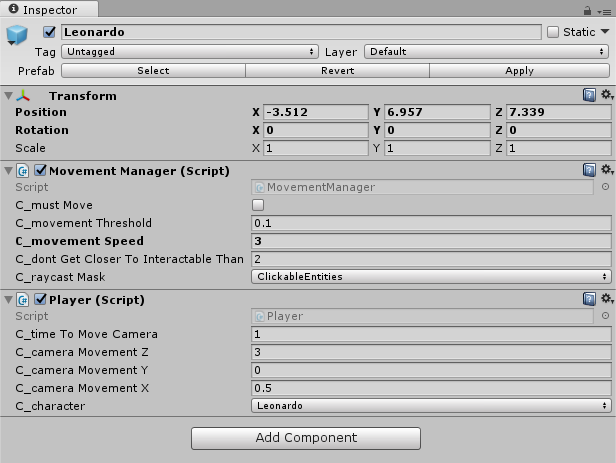
\includegraphics[scale=1]{imagenes/GameobjectsAndComponents.png}
\caption{Vista del editor de Unity3D donde se pueden ver los componentes de un Gameobject}
\label{gameobjectComponents}
\end{center}
\end{figure}

Como se ha mencionado anteriormente el componente \textquote{Transform} es obligatorio en todos \textquote{Gameobjects}. También se pueden ver otros dos componentes, \textquote{Movement Manager} y \textquote{Player}, que han sido creados por el desarrollador.
Dichos componentes dotan a la entidad, que en este caso es el personaje controlable por el jugador, de las características que lo hacen único. Entre otras cosas le dan la habilidad de reaccionar ante los inputs del usuario y moverse por el escenario. También se pueden observar una serie de variables con parámetros. Dado que cada instancia de los componentes es única para la entidad que lo agrega, se pueden personalizar para que incluso entre entidades con los mismos componentes se comporten de manera diferente.

En la siguiente imagen (ver fig. \ref{diagramaClasesUnity}) se puede observar un diagrama de clases que muestra la estructura que compone el sistema de componentes y los Gameobjects.

\begin{figure}[H]
\begin{center}
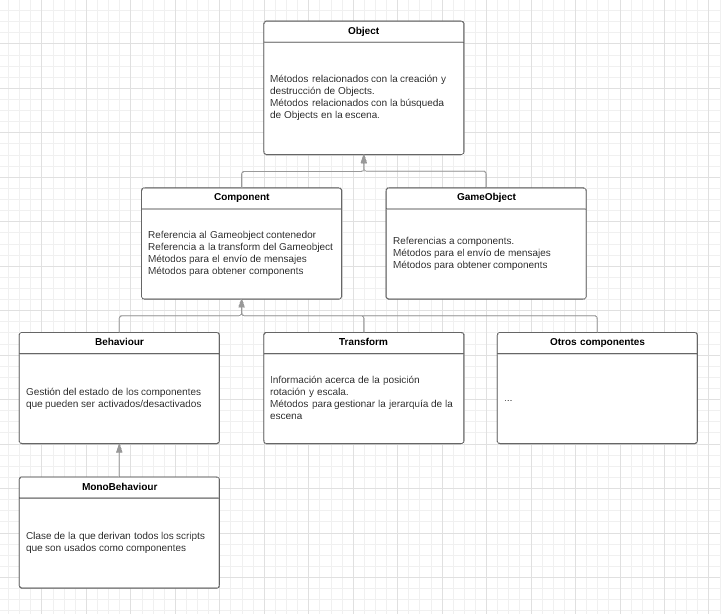
\includegraphics[scale=1]{imagenes/diagramaClasesUnity.png}
\caption{Diagrama de clases de Unity3D}
\label{diagramaClasesUnity}
\end{center}
\end{figure}

Los componentes que provee Unity3D derivan de la clase Component. En el caso de la imagen solo aparece el componente \textquote{Transform}, pero hay muchos más como \textquote{Renderer}, \textquote{Rigidbody}, \textquote{Collider}, etc. En la clase especializada cada componente contendrá la lógica necesaria para desempeñar su función, y el la clase Component se referenciará al \textquote{GameObject} que lo contiene. Cabe notar que un componente no puede existir de forma independiente. Debe estar siempre asociado a una entidad.

La clase MonoBehaviour es también muy importante ya que es la clase base para los scripts creados por los desarrollares. Cualquier fragmento de código que se desee añadir como componente a una entidad deberá heredar de dicha clase. 

Por supuesto se pueden escribir scripts que no hereden de la clase MonoBehaviour, pero en ese caso no podrán ser asignados como componentes a una entidad. Sin embargo no dejan de ser útiles ya que pueden ser usados como POCO \footnote{https://es.wikipedia.org/wiki/Plain\_Old\_CLR\_Object}, definir interfaces, contener lógica o cualquier otra cosa que el desarrollador desee. 

En última instancia los scripts que no heredan de MonoBehaviour deben de ser utilizados desde un script que sí lo haga, ya que este es el único punto de entrada que tienen hacia el sistema de Unity3D.

El último aspecto de la arquitectura que se comentará es el bucle de juego: una parte fundamenta de cualquier videojuego.
El bucle de juego es la parte software más importante en cualquier videojuego. En él se ejecutan las tareas que hacen que el juego 'esté vivo'.
En el siguiente fragmento de código (ver fig. \ref{bucleDeJuego}) se presenta un ejemplo de bucle de juego básico:

\begin{lstlisting}[caption={Código de bucle de juego básico},label=bucleDeJuego]
while(true)
{
	ProcesarInput();
	ActualizarJuego();
	Renderizar();
}
\end{lstlisting}

En este fragmento de código se pueden observar las tres tareas fundamentales de las que se compone cualquier videojuego:

\begin{itemize}
	\item Procesar input: consiste en capturar la interacción del usuario con el sistema mediante el hardware. En esta etapa se puede aplicar algún tipo de filtrado sobre dicho input.
	\item Actualizar juego: se actualiza el estado del juego. Esto consiste en actualizar IA, realizar las acciones del personaje, actualizar el mundo, efectos de objetos, etc.
	\item Renderizar: los elementos del juego se procesan para ser dibujados en la pantalla.
\end{itemize}

El ejemplo de bucle mostrado anteriormente es tremendamente básico pero sirve para explicar las bases de un bucle de juego. Probablemente ningún videojuego moderno lo utilice ya que tiene múltiples inconvenientes como que la frecuencia de actualización del juego dependerá de la carga de trabajo y del rendimiento del sistema que la procese. Actualmente existen variaciones del bucle que solucionan este problema, pero son temas que quedan fuera del alcance de este proyecto.

En la siguiente imagen (ver fig. \ref{bucleUnity}) se puede observar el bucle de juego utilizado por el motor Unity3D, y evidentemente por el juego creado para este proyecto:

\begin{figure}[H]
\begin{center}
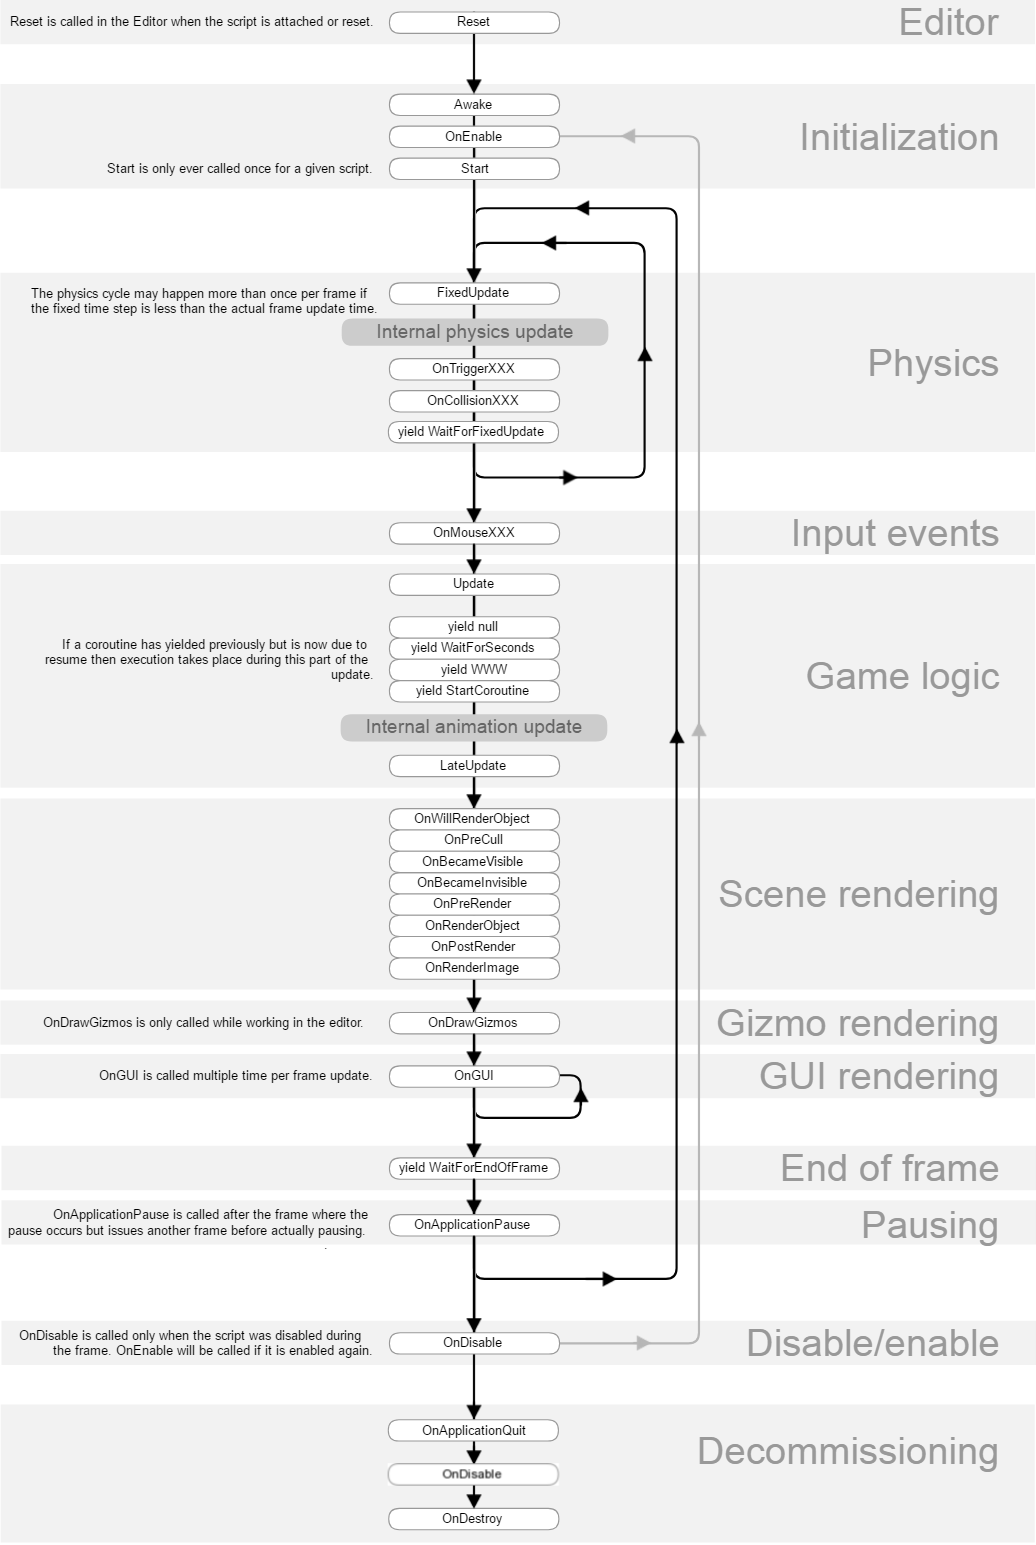
\includegraphics[scale=0.55]{imagenes/bucleUnity.png}
\caption{Bucle de juego del motor Unity3D}
\label{bucleUnity}
\end{center}
\end{figure}

En la imagen se pueden observar las 3 fases clave del bucle de juego: la captura de acciones del jugador, que se produce en la parte denominada como \textquote{Input Events}; la actualización del mundo de juego que se lleva a cabo en \textquote{Physics} y \textquote{Game logic}; finalmente el dibujado del mundo, que se produce en \textquote{Scene rendering}, \textquote{Gizmo rendering} y \textquote{GUI rendering}.


\subsection{Arquitectura del juego}

A continuación se describirá la arquitectura utilizada para desarrollar los componentes más importantes del juego. Estos son: el sistema de conversaciones y el sistema de escenarios. %y el sistema de cambio de personajes , el sistema de movimiento,

\subsubsection{Sistema de conversaciones}

El sistema de conversaciones es el más importante del juego ya que los diálogos con los personajes del juego son el hilo conductor de este.

Los diálogos en lugar de estar insertados directamente en el código se almacenan en ficheros de texto plano independientes. Esto permite que se puedan modificar los diálogos sin tener que recompilar el código del juego. Además permite que cualquier persona sin conocimientos de programación escriba diálogos.

Cada diálogo es un archivo que sigue el formato JSON \footnote{https://geekytheory.com/json-i-que-es-y-para-que-sirve-json}. Las conversaciones tienen una estructura arbórea donde los nodos representan la parte del diálogo correspondiente al NPC y las ramas salientes de dicho nodo representan las posibles contestaciones. La representación de una conversación en el formato JSON sigue la estructura que se puede ver en la siguiente imagen (ver fig. \ref{jsonFormat}).

\begin{figure}[H]
\begin{center}
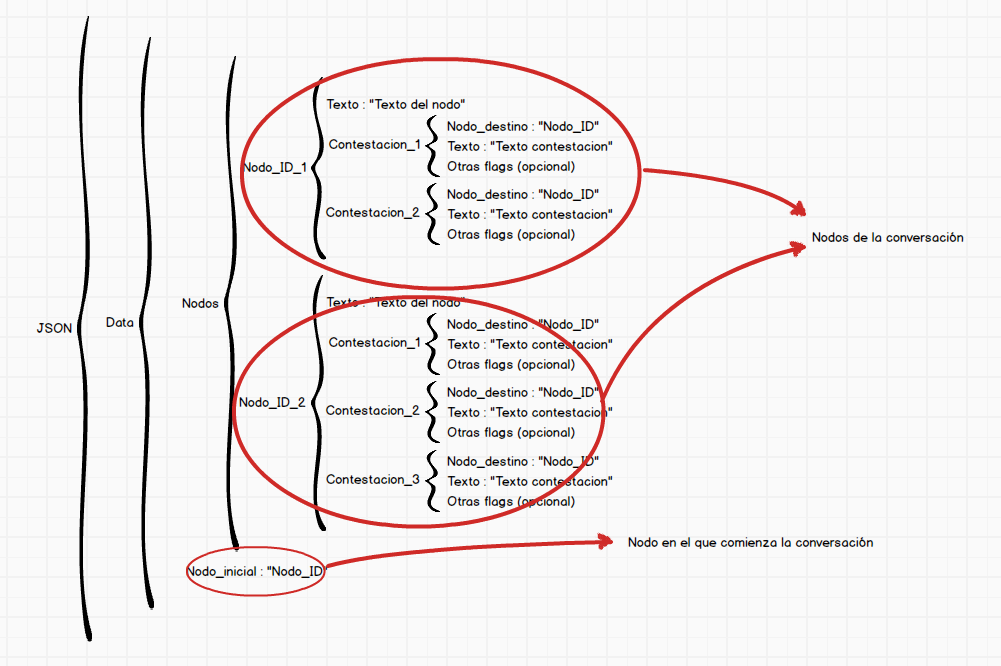
\includegraphics[scale=0.57]{imagenes/jsonFormat.png}
\caption{Representación del formato utilizado para los ficheros de diálogo}
\label{jsonFormat}
\end{center}
\end{figure}

Como se puede observar, los datos contenidos en el JSON son un array de objetos Nodo y un string que indica el nodo inicial de la conversación. 

Los objetos Nodos están indentificados por una cadena de texto que se compone de las tres primeras palabras del diálogo.Cada Nodo contiene el texto del NPC y las posibles contestaciones que el jugador le puede dar.

Las contestaciones se componen de el identificador del nodo al que conduce dicha contestación y el texto de la contestación en sí. Además puede contener ,o no, diferentes \textquote{flags} que le dan a la elección una funcionalidad extra. Entre las \textquote{flags} disponibles se encuentran la de acabar la conversación, desbloquear un objetivo o desbloquear un logro.

Para la creación de los ficheros de diálogos se puede escribir el JSON manualmente rellenando con los datos deseados o se puede utilizar la herramienta inklewritter \footnote{http://www.inklestudios.com/inklewriter/}. Dicha herramienta presenta una forma más sencilla de escribir conversaciones de múltiple respuesta (ver fig. \ref{inklewritter}). Además cuenta con la posibilidad de exportar el trabajo final a un fichero de texto en formato JSON. El parser JSON del videojuego está construido específicamente para poder procesar los diálogos construidos con inklewritter.

\begin{figure}[H]
\begin{center}
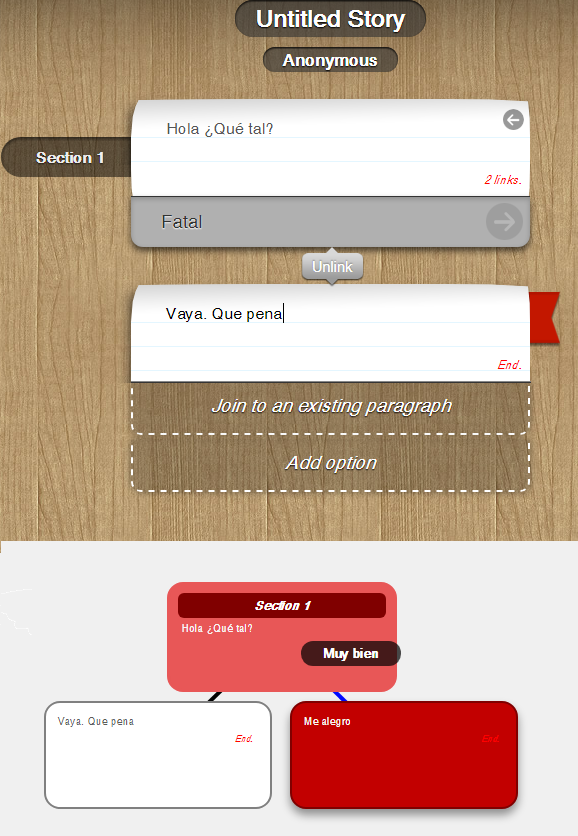
\includegraphics[scale=0.7]{imagenes/inklewritter.png}
\caption{Herramienta inklewritter}
\label{inklewritter}
\end{center}
\end{figure}

Para explicar la arquitectura del sistema de conversaciones se emplearán sendos diagramas de secuencia: uno para explicar el proceso de iniciar una conversación y otro para explicar el proceso de selección de contestaciones.

En el siguiente diagrama (ver fig. \ref{nuevaConversFlujo}) se ve el flujo de código necesario para iniciar una conversación. 

\begin{figure}[H]
\begin{center}
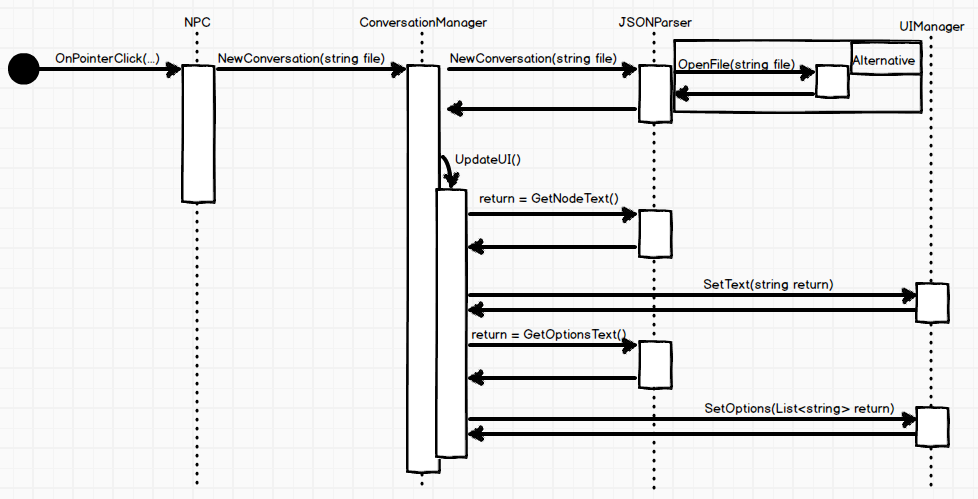
\includegraphics[scale=0.55]{imagenes/nuevaConversFlujo.png}
\caption{Diagrama de flujo nueva conversación}
\label{nuevaConversFlujo}
\end{center}
\end{figure}

No se ha indicado en el diagrama pero para el tratamiento JSON del fichero y para todas las operaciones JSON se utiliza la librería SimpleJSON \footnote{http://wiki.unity3d.com/index.php/SimpleJSON}.


El punto de entrada es el click del jugador en un NPC. Previamente el NPC se habrá registrado en el ConversationManager, de forma que el NPC guarda en un delegado el método NewConversation(string) del ConversationManager.

Cuando se le pide al ConversationManager que inicie una nueva conversación, el NPC le pasa por parámetro la ruta del fichero en la que está almacenado su diálogo con el personaje que está controlando el jugador en ese momento. El ConversationManager informará al JSONParser de que se debe iniciar una nueva conversación, y este será el encargado de leer y parsear el fichero o de abrir una de las conversaciones que tiene almacenadas.

Una vez informado el JSONParser, el ConversationManager le pedirá el texto del nodo actual de la conversación y el texto de las posibles respuestas. Una vez tenga esa información se la pasará al UIManager que se encarga de la interacción con los elementos gráficos de la interfaz.

En este arquitectura se ha seguido un diseño inspirado en el patrón Model-view-Controller \footnote{https://es.wikipedia.org/wiki/Modelo-vista-controlador}. Para ello todas las referencias a los elementos de la interfaz y los métodos de interacción con los mismos se han encapsulado en la clase llama UIManager. El acceso a los datos de las conversaciones, la gestión del estado de las mismas y la lectura de los ficheros de diálogos se guardan en la clase JSONParser, que además utiliza la librería SimpleJSON. En cuanto al punto de encuentro entre los datos y la interfaz, se emplea la clase ConversationManager para sincronizar las operaciones entre las otras dos clases y para proveer un punto de entrada al sistema de conversaciones.

Una vez abierta la conversación es necesario actualizar el juego cada vez que el jugador selecciona una respuesta. El funcionamiento de esta mecánica es muy similar y utiliza los mismos componentes que el sistema anterior.
En el siguiente diagrama de flujo (ver fig. \ref{respuestaFlujo}) se explica el proceso.

\begin{figure}[H]
\begin{center}
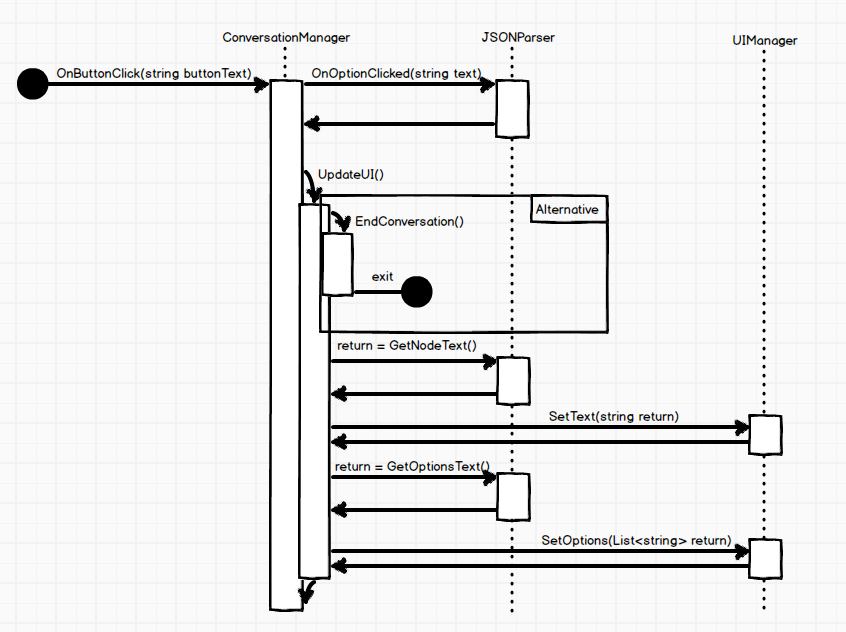
\includegraphics[scale=0.55]{imagenes/respuestaFlujo.png}
\caption{Diagrama de flujo de selección de respuesta}
\label{respuestaFlujo}
\end{center}
\end{figure}

\subsubsection{Sistema de escenarios}

A lo largo del juego se puede navegar por diferentes escenarios. Por temas de eficiencia y debido a que cada escenario tiene características únicas se han agrupado según la temática. En lugar de tener un gran escenario con montones de mallas correspondientes a los edificios y los personajes, solo están activos los Gameobjects correspondientes al escenario actual, los demás están desactivados (que no eliminados). En los escenarios hay puertas que al ser clicadas transportan al personaje activo hacia el escenario al que conduce la puerta. 

En el inspector de escena de Unity3D dichos escenarios lucen como se en la siguiente imagen (ver fig. \ref{unityScenarios}).

\begin{figure}[H]
\begin{center}
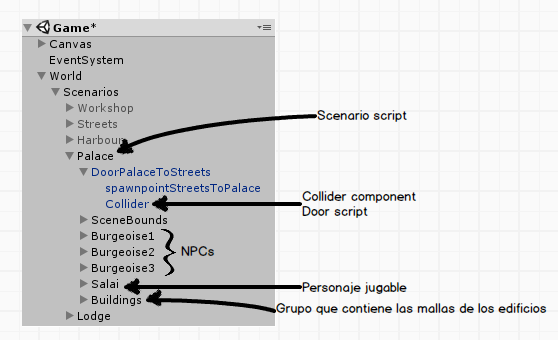
\includegraphics[scale=1]{imagenes/unityScenarios.png}
\caption{Vista de los escenarios en el inspector de Unity3D}
\label{unityScenarios}
\end{center}
\end{figure}

Como se puede observar algunos Gameobjects de la escena contienen scripts y componentes (otros Gameobjects tambien pero se han omitido para mayor simplicidad). En el siguiente diagrama de clases (ver fig. \ref{sceneClassDiagram}) se muestra la estructura de estos scripts y posteriormente se explicará su funcionamiento y utilidad.

\begin{figure}[H]
\begin{center}
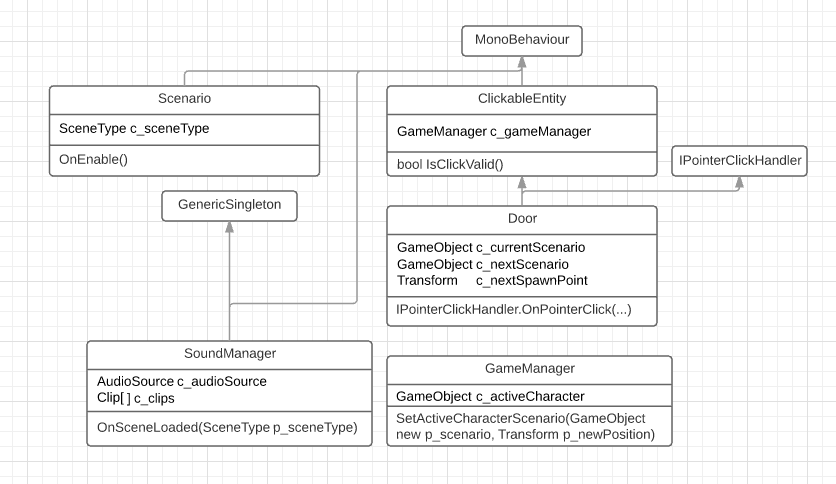
\includegraphics[scale=0.75]{imagenes/sceneClassDiagram.PNG}
\caption{Diagrama de clases del sistema de escenarios}
\label{sceneClassDiagram}
\end{center}
\end{figure}

El elemento central de todo el sistema de escenarios es la puerta. El nombre del Gameobject puerta sigue una notación que indica el escenario destino y origen. En el caso de la imagen anterior (ver fig. \ref{unityScenarios}) se puede observar que la puerta lleva del Palacio (el escenario activo) a Las calles (un escenario desactivado).

El método IPointerClickHandler.OnPointerClick(...), heredado de la interfaz IPointerClickHandler que provee Unity3D, es llamado cuando se hace click en el componente Collider asociado a la puerta. Posteriormente se comprobará que el click es válido (el jugador no está muy lejos por ejemplo) con el método heredado IsClickValid(). Finalmente se notificará al GameManager de que se quiere hacer un cambio de escena y se le suministrará el Gameobject que contiene la nueva escena y la posición de inicio para el jugador.

El sistema de escenarios se encarga también de gestionar la pista de audio que se reproduce a modo de música ambiental. En el objeto raíz de cada escenario se encuentra un script que hace uso del método provisto por Unity3D, OnEnable(). Dicho método es llamado cada vez que se activa un escenario. Desde el método OnEnable() se notifica al SoundManager, que es accesible de forma global ya que implementa el patrón Singleton, el nuevo escenario activado. El SoundManager dispone de un clip de sonido por cada escenario y cuando recibe el tipo del nuevo escenario cambia el clip de sonido reproducido por el componente AudioSource.

\subsection{Storytelling}

El storytelling es una parte fundamental del videojuego creado. Uno de los aspectos que hacen diferente a Da Vinci Startup es que en lugar de saturar al usuario con insufribles lecciones de teoría sobre emprendimiento, se aprende a la vez que se juega. Eso no significa que el conocimiento técnico no esté presente. La diferencia es que el conocimiento se adquiere a lo largo de la historia que los NPCs cuentan y que el jugador experimenta. De este modo conceptos como el "networking" no son solo palabras en un manual, si no que el jugador deberá utilizarlo a lo largo del juego para lograr los objetivos que le llevarán a completar el mismo.

\subsubsection{Guion literario}

Previamente a la implementación del videojuego se escribió un guion literario. Dicho guion explica la historia a desarrollar en el juego de una forma más narrativa, como si de un libro o historia se tratase.
Dicho guion se encuentra en el apartado \nameref{guionLiterario} incluido en el \nameref{GDD}. Dicha historia es una historia ficticia en la que un mentor guía a Leonardo durante la construcción de la startup.

\subsubsection{Guion técnico}

Además del guion literario se ha elaborado un guion técnico en el que se especifican las diferentes pantallas que componen el menú principal junto con los mockups que las definen. El diagrama de pantallas del menú principal se puede encontrar en el apartado \nameref{guionTecnico} del Anexo I.


Se han elaborado también los mockups que definen a los diferentes menús disponibles durante la partida. Se incluye además una explicación del funcionamiento de cada elemento que se puede consultar en el apartado \nameref{mockupsJuego} del Anexo I.


En cuanto a los personajes disponibles en el juego, tanto controlables como no controlables, y los escenarios se dispone de una descripción detallada en los apartados \nameref{personajes} y \nameref{descripcionEscenarios} respectivamente.
\chapter{Resultados}

Se  puede afirmar que llegados a la finalización del desarrollo del sistema se ha obtenido un resultado satisfactorio. Se han implementado casi todos los requisitos del sistema y el videojuego provee de una experiencia de juego completa.

Se ha completado también el objetivo principal del proyecto: crear un videojuego que eduque sobre emprendimiento y \textquote{LeanStartup}. Se ha usado el storytelling para que el jugador reciba información sobre \textquote{Lean startup} al conversar con los NPCs del juego (ver fig. \ref{dialogo}).

\begin{figure}
\begin{center}
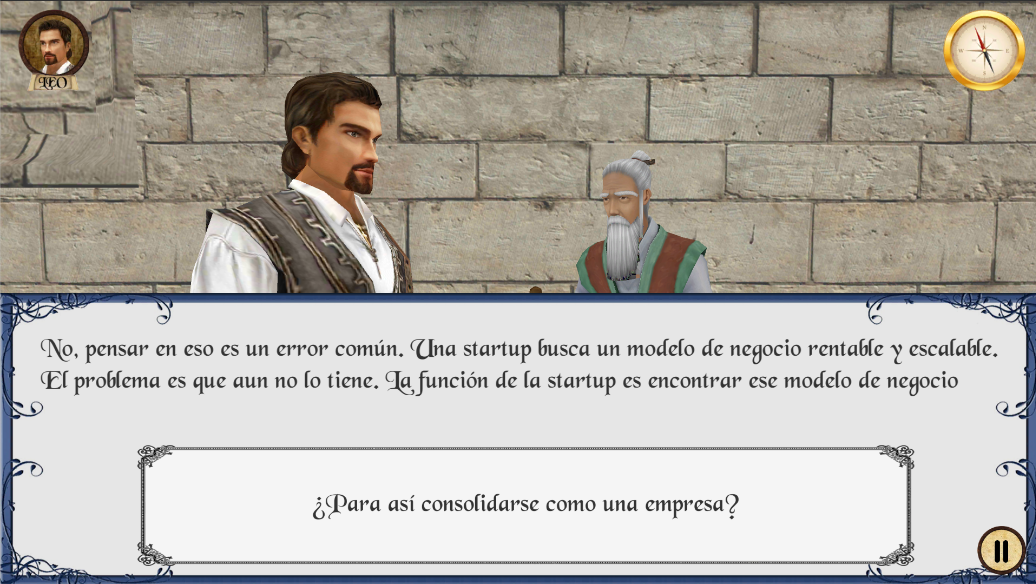
\includegraphics[scale=0.5]{imagenes/dialogo.png}
\caption{Jugador dialogando con NPC en Da Vinci Startu.  Fuente: elaboración propiap}
\label{dialogo}
\end{center}
\end{figure}

El desarrollo del proyecto se ha llevado a cabo con Unity3D y utilizando el lenguaje de programación C\#. Se han ampliado enormemente los conocimientos sobre ambas herramientas y se han aprendido muchas técnicas de desarrollo sobre las mismas.

Se han creado también varios  escenarios por los que el jugador puede transitar libremente y moverse de uno a otro(ver fig. \ref{escenarios}).

\begin{figure}
\begin{center}
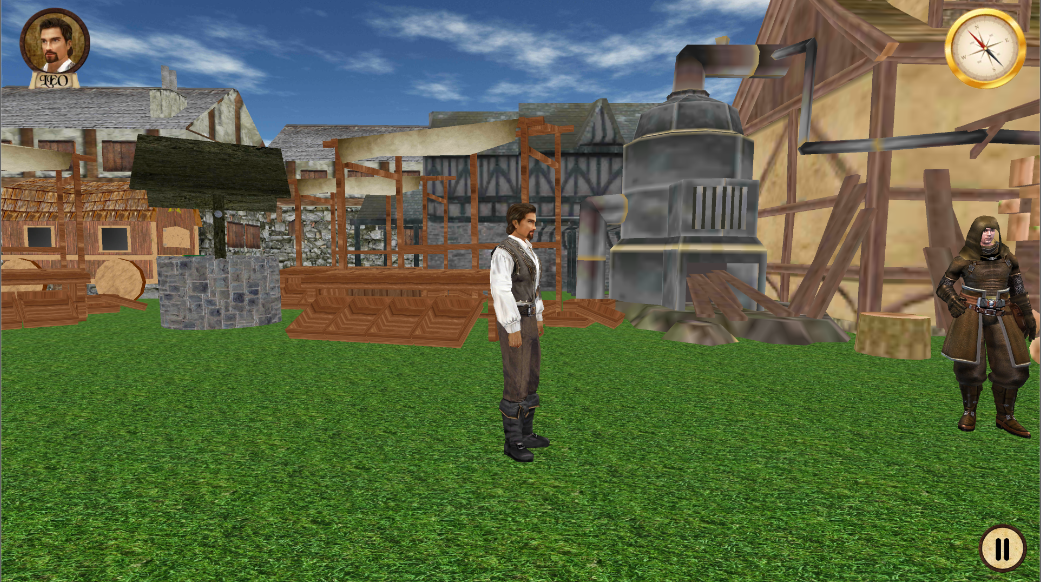
\includegraphics[scale=0.5]{imagenes/escenarios.png}
\caption{Jugador en el escenario Calles de Florencia}
\label{escenarios}
\end{center}
\end{figure}

Se ha implementado también el sistema de interfaces propuesto, ofreciendo al jugador  toda la funcionalidad necesaria pero sin comprometer la jugabilidad. Entre las interfaces creadas se encuentran  el selector de personajes, el indicador de objetivos y el menu de pausa (ver fig. \ref{iu}). Además se ha creado un menú principal con varias ventanas en las que visualizar información como los logros, las opciones, información sobre el desarrollador, etc (ver fig. \ref{titulo}).

\begin{figure}
\begin{center}
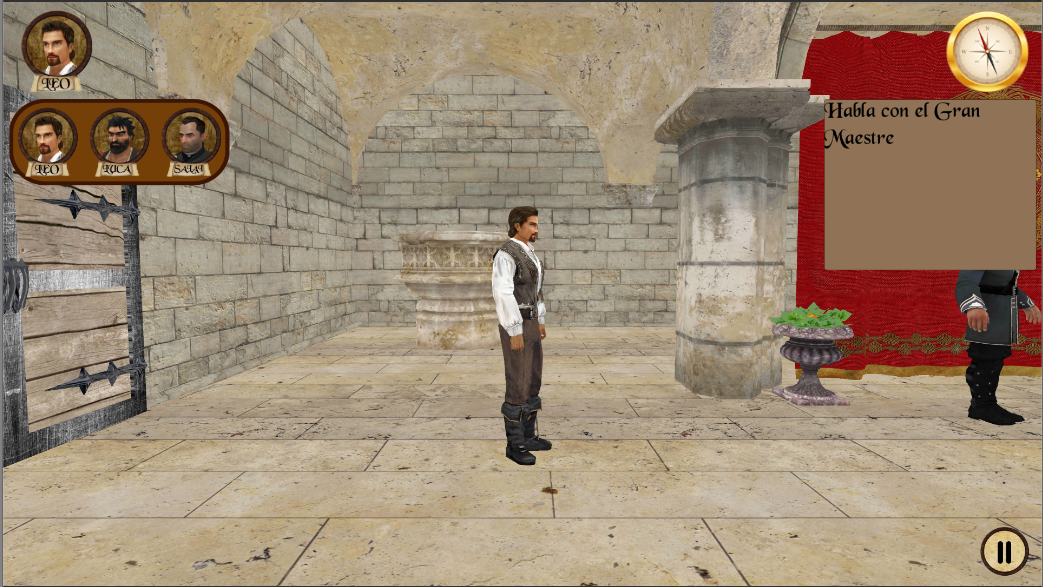
\includegraphics[scale=0.5]{imagenes/iu.png}
\caption{Interfaz de usuario durante la partida con los menús desplegados.  Fuente: elaboración propia}
\label{iu}
\end{center}
\end{figure}

\begin{figure}
\begin{center}

\includegraphics[scale=0.5]{imagenes/titulo.png}
\caption{Menú principal del juego.  Fuente: elaboración propia}
\label{titulo}
\end{center}
\end{figure}

En cuanto a los objetivos que no se han podido cumplir: no se han podido crear los modelos 3D para el juego. En su lugar se han tenido que utilizar recursos que se ofrecen de forma gratuita. Tampoco se han podido cumplir los requisitos correspondientes a Guardar juego (RF-SYS-08) y Cargar juego (RF-SYS-09). En cualquier caso no son requisitos que comprometan la experiencia de juego y que impidan el transcurso de una partida. 

En resumen, el producto creado no es un juego finalizado, pero si que se puede considerar un Mínimo producto viable que se podría enseñar a inversores que estén interesados en apoyar el desarrollo del juego. O mostrar a personas que podrían estar interesadas en unirse al equipo. También es el primer paso para poder probar el juego con usuarios reales y seguir trabajando acorde a las opiniones de estos. 

Para concluir, el producto creado cumple perfectamente con lo esperado del mismo. Ofrece una experiencia de juego completa y contiene todos los elementos planeados para el juego. Es un punto de partida perfecto para reunir un equipo, buscar financiación y convertirlo en un juego que se pueda comercializar.
%input{capitulos/conclusiones}

%\nocite{*} %incluye TODOS los documentos de la base de datos bibliográfica sean o no citados en el texto
\bibliography{bibliografia/bibliografia}
\addcontentsline{toc}{chapter}{Bibliografía} %sustituir bibliografía con el nombre del fichero bibtex con la bibliografía
\bibliographystyle{apalike}
%
\appendix
\chapter{Anexo I}
Aquí vendría en anexo I 
%\input{glosario/entradas_glosario}
% \addcontentsline{toc}{chapter}{Glosario} %si se usa glosario hay que añadirlo al índice
% \printglossary %muestra el glosario

\end{document}
